% !TeX program = xelatex
% 2026 CUMCM C题：微网与外部电网电力调控策略
% 编译：latexmk -xelatex cumcm.tex
\documentclass[zihao=-4,a4paper,UTF8,fontset=none]{ctexart}

% template
\usepackage{cumcm2026}

% set English and Number font
\setmainfont{TimesNewRoman.ttf}[
  Path=fonts/,
  BoldFont=TimesNewRomanBold.ttf,
  ItalicFont=TimesNewRomanItalic.ttf,
  BoldItalicFont=TimesNewRomanBoldItalic.ttf
]

% set Chinese font
\setCJKmainfont[
  Path=fonts/,
  BoldFont=SimHei.ttf
]{SimSun.ttc}

\setCJKfamilyfont{zhsong}[
  Path=fonts/
]{SimSun.ttc}

\setCJKfamilyfont{zhhei}[
  Path=fonts/
]{SimHei.ttf}

\providecommand{\songti}{}
\providecommand{\heiti}{}
\renewcommand{\songti}{\CJKfamily{zhsong}}
\renewcommand{\heiti}{\CJKfamily{zhhei}}

\usepackage{tikz}
\usetikzlibrary{arrows.meta, positioning, calc}

%--------------------------------------------------------------------
%以上不要动
\title{基于多层随机优化的微网购电决策与调控策略}
\newcommand{\keywords}{微电网；两阶段随机规划；储能调度；滚动优化；信息融合}

\begin{document}

\maketitle

\begin{cumcmabstract}
本文针对微网在分时电价与光伏出力不确定性下的购电决策问题，以购电费用最小为目标，建立\textbf{``预测—计划—调整—执行''多层随机优化模型体系}，四问共用同一框架并随信息结构递进扩展，全部模型在全年真实数据上严格因果回测，并经\textbf{九组替代策略对照实验}验证方法有效性。

针对问题一，建立\textbf{日循环线性规划模型}，决策 144 个 10 分钟时段的购电与充放电量，约束涵盖充放电功率上限（5000 kW）、荷电状态安全区间（1200--10800 kWh）与日循环平衡，HiGHS 求解器求得全局最优：全天购电量 59482.70 kWh，购电费 \textbf{35126.85 元，较无储能基准降低 26.90\%}；策略呈``低谷充电、双峰放电''套利结构，对偶分析给出边际供电成本曲线与储能容量影子价格（最大 0.2017 元/kWh）。

针对问题二，构建\textbf{加权混合预测器}（负载取同星期近 3 周加权均值、光伏取近 7 日加权均值，净负荷 MAE 266.1 kW），建立\textbf{两阶段随机规划（场景法）计划模型}——第一阶段决策计划购电量、第二阶段以历史误差场景刻画期望罚金；执行层用\textbf{滚动实时线性规划}将紧急购电转移至低价时段。全年（2025.2.1--12.31）总费用 \textbf{1387.90 万元，较无储能基准降低 15.41\%}，距理想先知基准仅 13.34\%。九组替代策略对照均未超过主策略，表明在所比较的策略空间内，``SAA 期望最优 + 缺口时滚动干预'取得了最低回测费用。

针对问题三，将官方预报与历史均值\textbf{按均方误差倒数加权组合}（光伏预测 MAE 由 197.5 降至 127.8 kW），并在 6/12/18 时进行\textbf{场景化滚动调整}——以新预报误差场景重解两阶段调整规划，偏差结算（少买退 50\%、超买 1.5 倍）线性化嵌入目标。总费用降至 \textbf{1347.60 万元}：信息融合贡献 11.0 万元，三次调整再省 \textbf{29.25 万元}并使紧急购电费下降 39\%。\textbf{结论是需要引入其他时刻的预报}：12 时预报（午后精度最高）单独贡献 21.31 万元，18 时调整的价值来自储能状态反馈渠道；且调整层必须与计划层保持同一随机优化视角，否则调整反而受损。

针对问题四，将电价路径替换为附件4（0.0076--1.7936 元/kWh）重算：问题二模型总费用 \textbf{1460.76 万元}，问题三模型 \textbf{1414.53 万元}。近零电价时段的免费充电与高峰深度放电使储能较无储能基准节省 288.13 万元（16.9\%），且\textbf{调整价值由 29.25 万元放大至 32.41 万元}，策略结构对电价体制稳健。

灵敏度分析表明：充放电效率 $\pm 0.05$ 对应费用变化 $\pm 3\%\sim4\%$；储能容量上限由 10800 降至 8640 kWh 时费用上升 5.1\%，升至 12000 kWh 时下降 2.2\%——容量是主导经济参数。报童理论最优分位数（$q^*=0.8$）与实测最优区间 $[0.7,0.8]$ 一致，验证了风险决策机制的合理性。

\cumcmkeywords{\keywords}
\end{cumcmabstract}

\section{问题重述}

\textbf{问题背景}。非孤岛式微网整合小区负载、光伏发电与储能设备，通过向外网购电满足用电需求。储能设备参数：最大容量 12000 kWh，充放电功率上限 5000 kW，荷电状态安全区间 $[1200, 10800]$ kWh，充放电效率 90\%，2025 年 1 月 1 日 0:00 初始电量 6000 kWh。调控目标：在满足负载的前提下最小化全天购电费用。

\textbf{数据条件}。附件1 提供某典型日的电价、负载与光伏预测（10 分钟粒度）；附件2 提供全年逐 10 分钟的实际负载与光伏功率；附件3 提供每天 0/6/12/18 时的光伏功率预报（覆盖未来 24 个整点）；附件4 提供全年实时电价。

\textbf{待解决问题}：
\begin{enumerate}
  \item \textbf{确定性环境}：电价与负载恒定、光伏预测已知，建立日循环的日前计划购电模型，给出典型日的购电与充放电结果；
  \item \textbf{预测误差环境}：电价恒定而负载与光伏逐日变化，计划购电量按计划量结算（take-or-pay），实际不足时以 5 倍电价紧急购电，建立逐日计划模型并评估全年效果；
  \item \textbf{多时点信息更新}：新增四次光伏预报，调减部分按 50\% 违约价结算、调增超出部分按 1.5 倍结算，建立含调整机制的购电模型，并论证是否需要引入其他时刻的预报；
  \item \textbf{波动电价}：电价实时波动，在波动电价下重新计算问题二与问题三。
\end{enumerate}

\section{问题分析}

\subsection{总体思路}

四个问题呈递进关系：决策环境从完全确定（问题一）到负载与光伏随机（问题二）、再到信息逐时更新（问题三）与电价波动（问题四），但核心决策结构一致——在每个决策时刻，基于可得信息确定未来 144 个 10 分钟时段的购电量与储能充放电量。为此，本文构建统一的三层框架：

\begin{enumerate}
  \item \textbf{计划层}：每天 0:00，基于当日负载与光伏的预测（信息集随问题递进而丰富）求解日前线性规划，得到计划购电量与充放电计划；
  \item \textbf{调整层}（问题三、四）：在 6/12/18 时利用新发布的光伏预报对剩余时段购电量进行滚动调整，调整成本由偏差结算规则刻画；
  \item \textbf{执行层}：购电量按计划（或调整后）数量结算并强制执行，储能充放电通过滚动实时 LP 调度——该 LP 在满足负载的约束下可自由分配充电、放电与紧急购电，其中紧急购电变量允许同时满足负载缺口与储能充电需求（题目未明确禁止紧急购电用于充电，本文将其作为 LP 的自然扩展）。
\end{enumerate}

问题一为确定性线性规划，可直接求得全局最优，并作为后续问题的基准；问题二的关键在于日前预测模型的构建与紧急购电机制的处理；问题三的关键在于将 50\%/1.5 倍的偏差结算规则线性化嵌入滚动调整模型；问题四将电价由固定曲线替换为波动路径，检验前述模型的适应性。总体技术路线见图~\ref{fig:route}。

\begin{figure}[H]
  \centering
  \begin{tikzpicture}[
    font=\small,
    dbox/.style={draw=black!60, rounded corners=1.5pt, fill=blue!7, align=center,
                 inner sep=2.5pt, minimum height=9.5mm},
    lbox/.style={draw=black!60, rounded corners=1.5pt, fill=orange!15, align=center,
                 inner sep=3.5pt, minimum height=8.5mm},
    obox/.style={draw=black!60, rounded corners=1.5pt, fill=green!9, align=center,
                 inner sep=3pt, minimum height=8.5mm},
    fl/.style={-{Stealth[length=1.8mm]}, semithick, black!55},
    lab/.style={font=\small\bfseries, black!75, align=center},
    ptag/.style={font=\footnotesize, black!65, align=left}
  ]
    % ---- 数据层 ----
    \node[dbox, minimum width=30mm] (a1) {附件1：典型日\\电价/负载/光伏};
    \node[dbox, minimum width=30mm, right=3.5mm of a1] (a2) {附件2：全年负载与\\光伏实际功率};
    \node[dbox, minimum width=30mm, right=3.5mm of a2] (a3) {附件3：光伏预报\\（0/6/12/18 时）};
    \node[dbox, minimum width=25mm, right=3.5mm of a3] (a4) {附件4：全年\\实时电价};
    \node[lab] at ($(a1.west)+(-6.5mm,0)$) {数\\[1pt]据\\[1pt]层};
    % ---- 预测层 ----
    \node[lbox, minimum width=46mm, anchor=north west] (p1) at ([yshift=-8mm]a1.south west)
      {负载预测：同星期近 3 周加权\\（MAE 169.1 kW）};
    \node[lbox, minimum width=46mm, anchor=north west] (p2) at ([xshift=4mm]p1.north east)
      {光伏预测：近 7 日均值；问题三与\\官方预报按均方误差倒数加权组合（MAE 127.8 kW）};
    \node[lbox, minimum width=40mm, anchor=north west] (p3) at ([xshift=4mm]p2.north east)
      {风险防范：报童分位数缓冲；\\升级为两阶段随机规划};
    \node[lab] at ($(p1.west)+(-6.5mm,0)$) {预\\[1pt]测\\[1pt]层};
    % ---- 计划层 ----
    \node[lbox, minimum width=140mm, anchor=north west] (plan) at ([yshift=-6mm]p1.south west)
      {计划层（每天 0:00）：日循环线性规划，$\min \sum_t p_t g_t$；
       约束：SOC 平衡与区间 $[1200,10800]$、功率 $\le 833.33$ kWh/槽、供需平衡、日循环};
    \node[lab] at ($(plan.west)+(-6.5mm,0)$) {计\\[1pt]划\\[1pt]层};
    % ---- 调整层 ----
    \node[lbox, minimum width=140mm, anchor=north west] (adj) at ([yshift=-5mm]plan.south west)
      {调整层（问题三/四，6/12/18 时）：新预报误差场景下的两阶段调整 LP；
       偏差结算线性化：结算 $= p a + 0.5p\,|a-g|$};
    \node[lab] at ($(adj.west)+(-6.5mm,0)$) {调\\[1pt]整\\[1pt]层};
    % ---- 执行层 ----
    \node[lbox, minimum width=140mm, anchor=north west] (exe) at ([yshift=-5mm]adj.south west)
      {执行层（每 10 分钟）：购电量锁定；盈余充电（越限弃电），缺口放电（越限 5 倍价紧急购电）；
       滚动实时 LP 将紧急购电转移至低价时段};
    \node[lab] at ($(exe.west)+(-6.5mm,0)$) {执\\[1pt]行\\[1pt]层};
    % ---- 输出与问题对应 ----
    \node[obox, minimum width=42mm, anchor=north east] (out) at ([yshift=-6mm]exe.south east)
      {结果输出：\\result1 $\sim$ result4-3.xlsx};
    \node[ptag, anchor=north west, text width=88mm] (prob) at ([yshift=-6mm]exe.south west)
      {问题一：计划层（确定环境）\\ 问题二：预测 + 计划 + 执行\\
       问题三：+ 调整层 + 信息融合\\ 问题四：电价路径替换为附件4};
    % ---- 箭头 ----
    \draw[fl] (a1.south) -- ++(0,-1.5mm) -| (p1.north);
    \draw[fl] (a2.south) -- ++(0,-1.5mm) -| (p2.north);
    \draw[fl] (a3.south) -- ++(0,-1.5mm) -| (p2.north east);
    \draw[fl] (a4.south) -- ++(0,-1.5mm) -| (p3.north);
    \draw[fl] (p1.south) -- (plan.north -| p1.south);
    \draw[fl] (p2.south) -- (plan.north -| p2.south);
    \draw[fl] (p3.south) -- (plan.north -| p3.south);
    \draw[fl] (plan.south) -- (adj.north);
    \draw[fl] (adj.south) -- (exe.north);
    \draw[fl] (exe.south) -- (out.north);
  \end{tikzpicture}
  \caption{总体技术路线：数据层—预测层—计划层—调整层—执行层}
  \label{fig:route}
\end{figure}

\subsection{数据探索性分析}

\textbf{负载周期结构}。小区负载呈显著的周内周期（图~\ref{fig:eda}(a)）：周一至周四与周日的日内形态相近（双峰结构，峰值约 5000 kW），而\textbf{周五与周六的负载仅为其余日的约 1/3}——星期效应可解释总方差的 85.3\%。这一发现直接指导了预测器设计（同星期加权）与场景选择策略。

\textbf{光伏季节性}。光伏日发电量呈明显的季节波动（图~\ref{fig:eda}(b)）：夏季（6--8 月）中位数约 7 万 kWh/日，冬季（12--2 月）仅约 3.5 万 kWh/日，且月内日间波动大（多云天气导致箱线图须较长），说明天气驱动的不确定性是光伏预测的核心挑战。

\textbf{电价模式}。固定电价呈``凌晨低谷—早高峰—午间小低谷—晚高峰''四段结构（图~\ref{fig:eda}(c)），峰谷比约 3.2:1；波动电价（附件4）在此基础上叠加随机扰动，波动范围 [0.008, 1.794] 元/kWh，峰谷差进一步拉大。

\textbf{净负荷分布}。全年净负荷呈\textbf{双峰分布}（图~\ref{fig:eda}(d)）：主峰约 3.5 MW（工作日白天光伏不足时段），次峰约 0（光伏充裕时段），负值（光伏过剩）时段占比约 15\%——储能需同时应对正向缺口（紧急购电风险）与负向过剩（弃电风险）。

\begin{figure}[H]
  \centering
  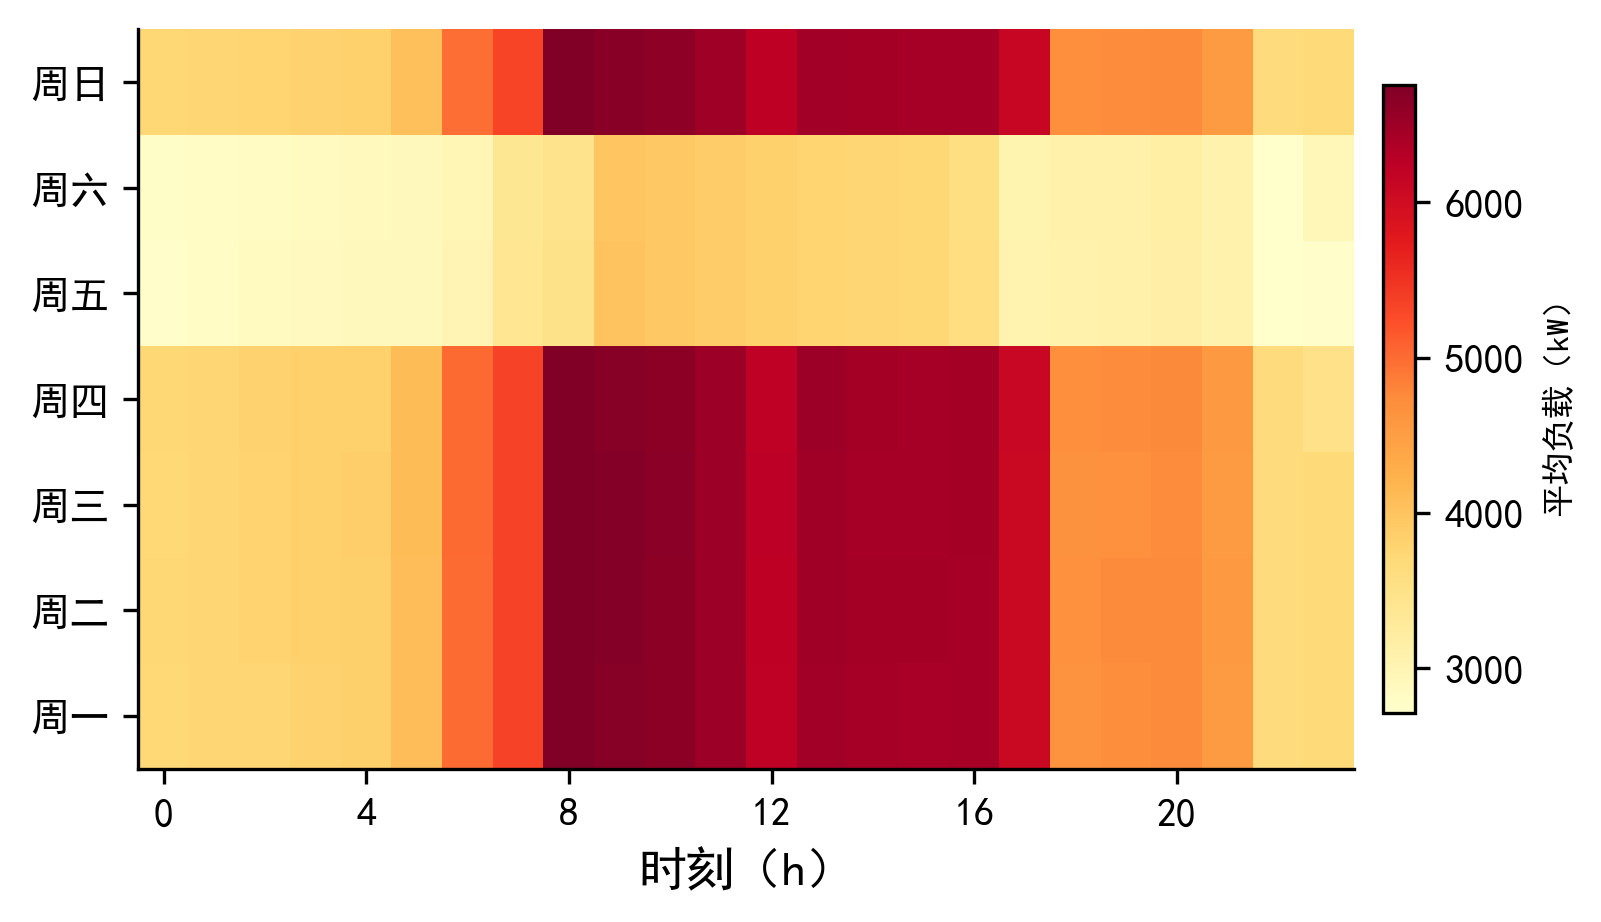
\includegraphics[width=0.95\textwidth]{figures/fig_eda_load_heatmap.png}\hfill
  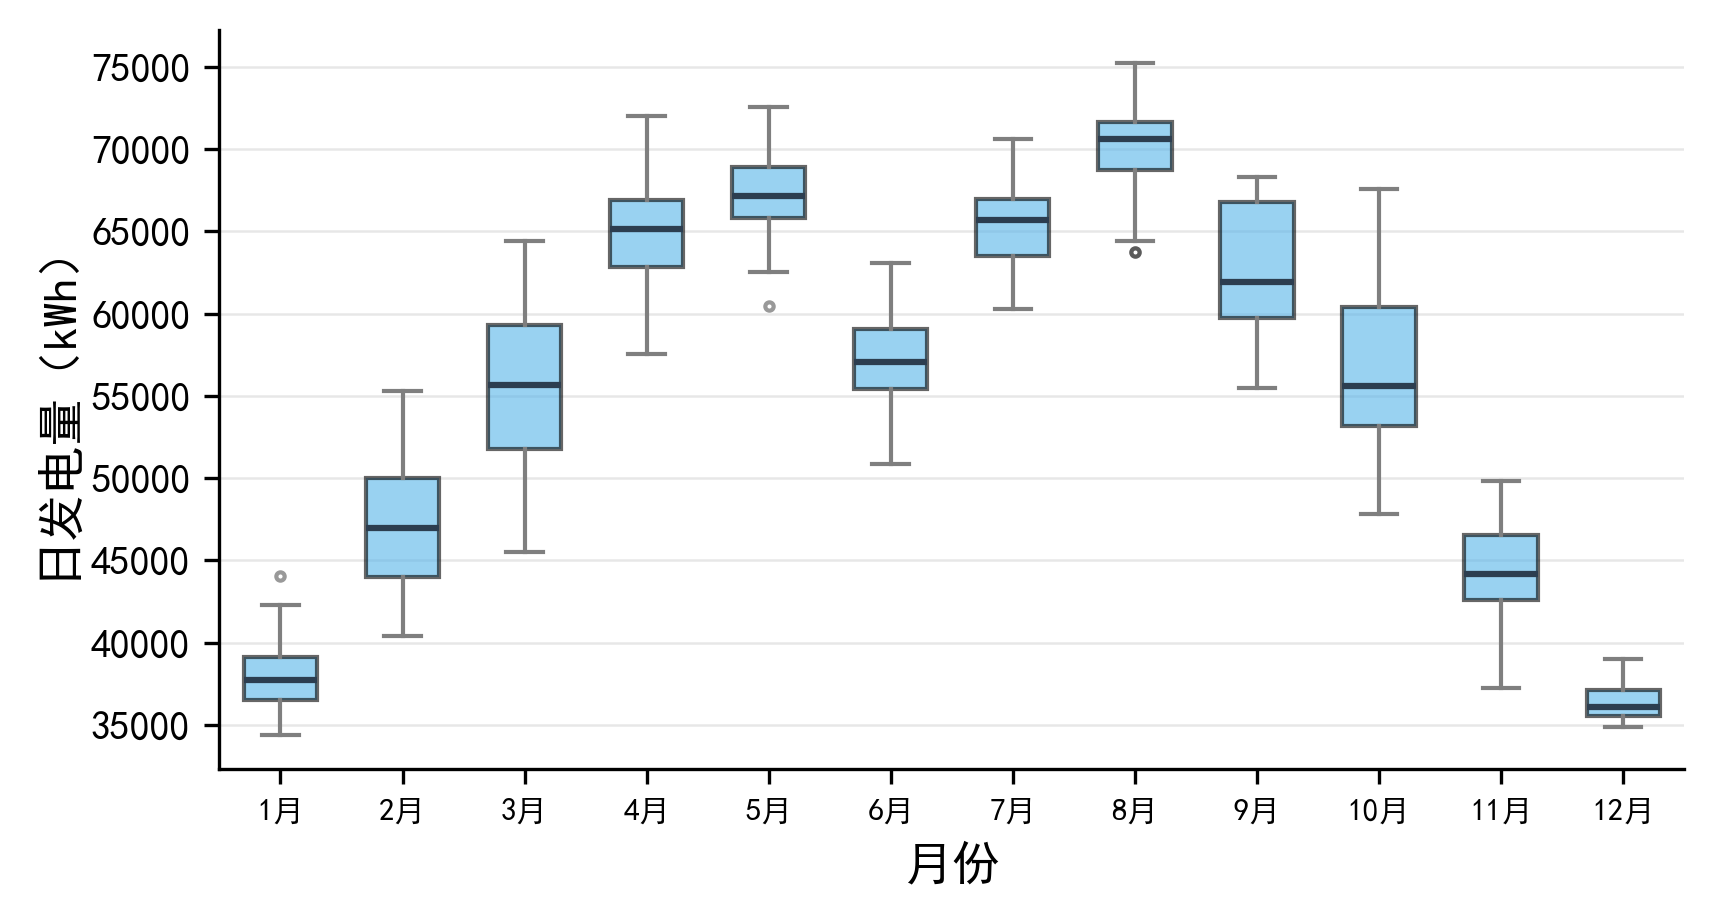
\includegraphics[width=0.95\textwidth]{figures/fig_eda_pv_monthly.png}
  \vfill
  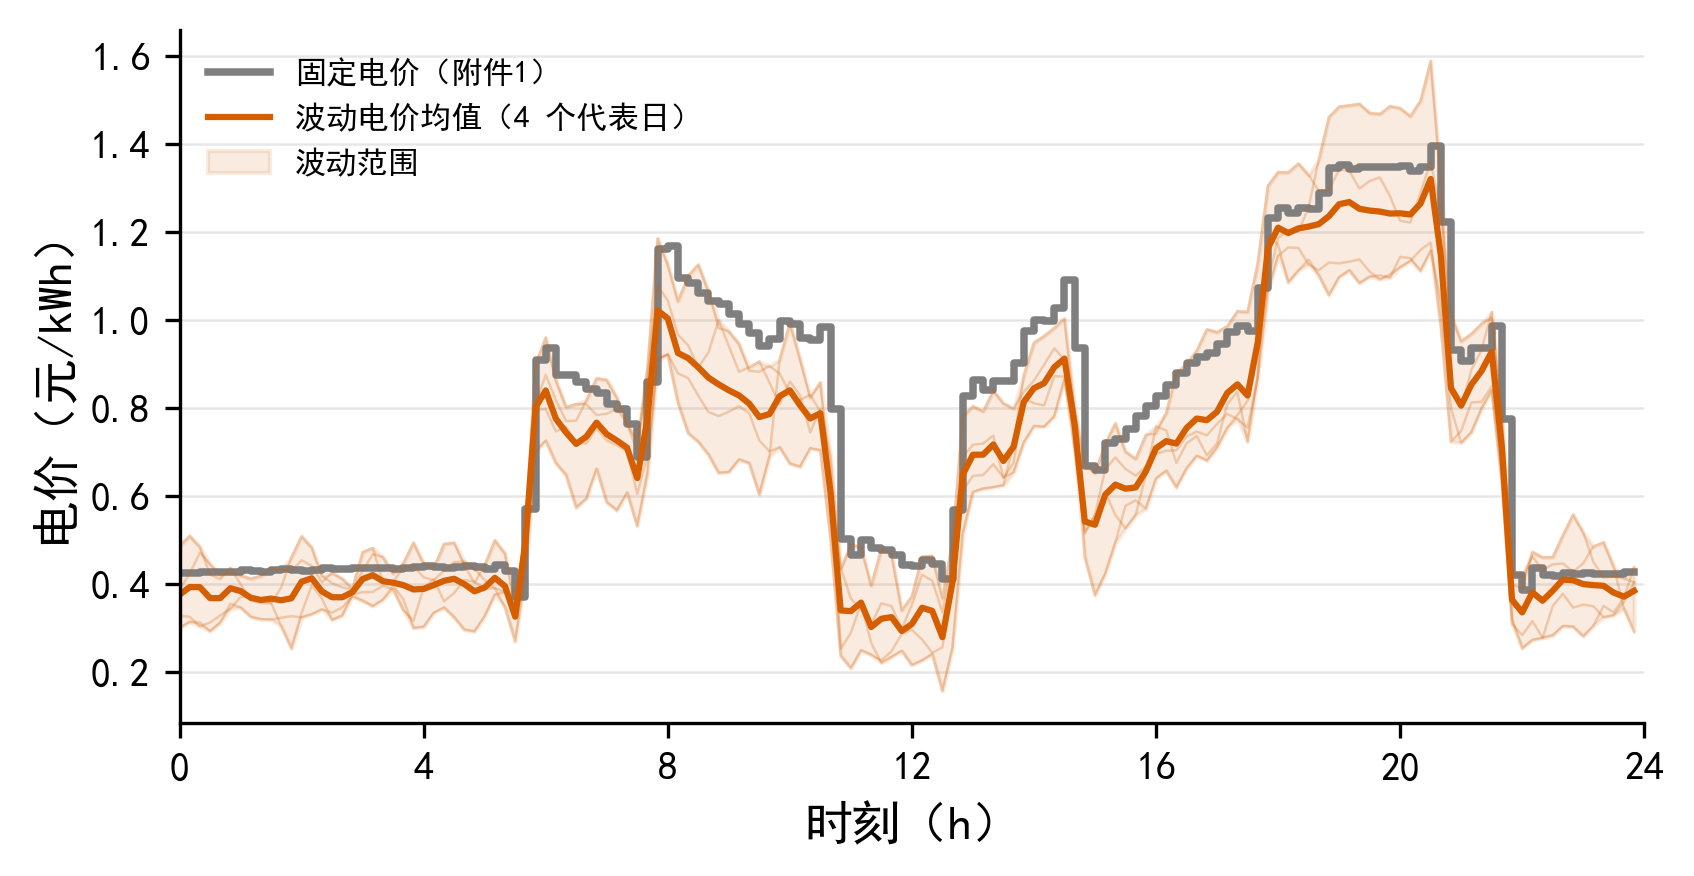
\includegraphics[width=0.95\textwidth]{figures/fig_eda_price.png}\hfill
  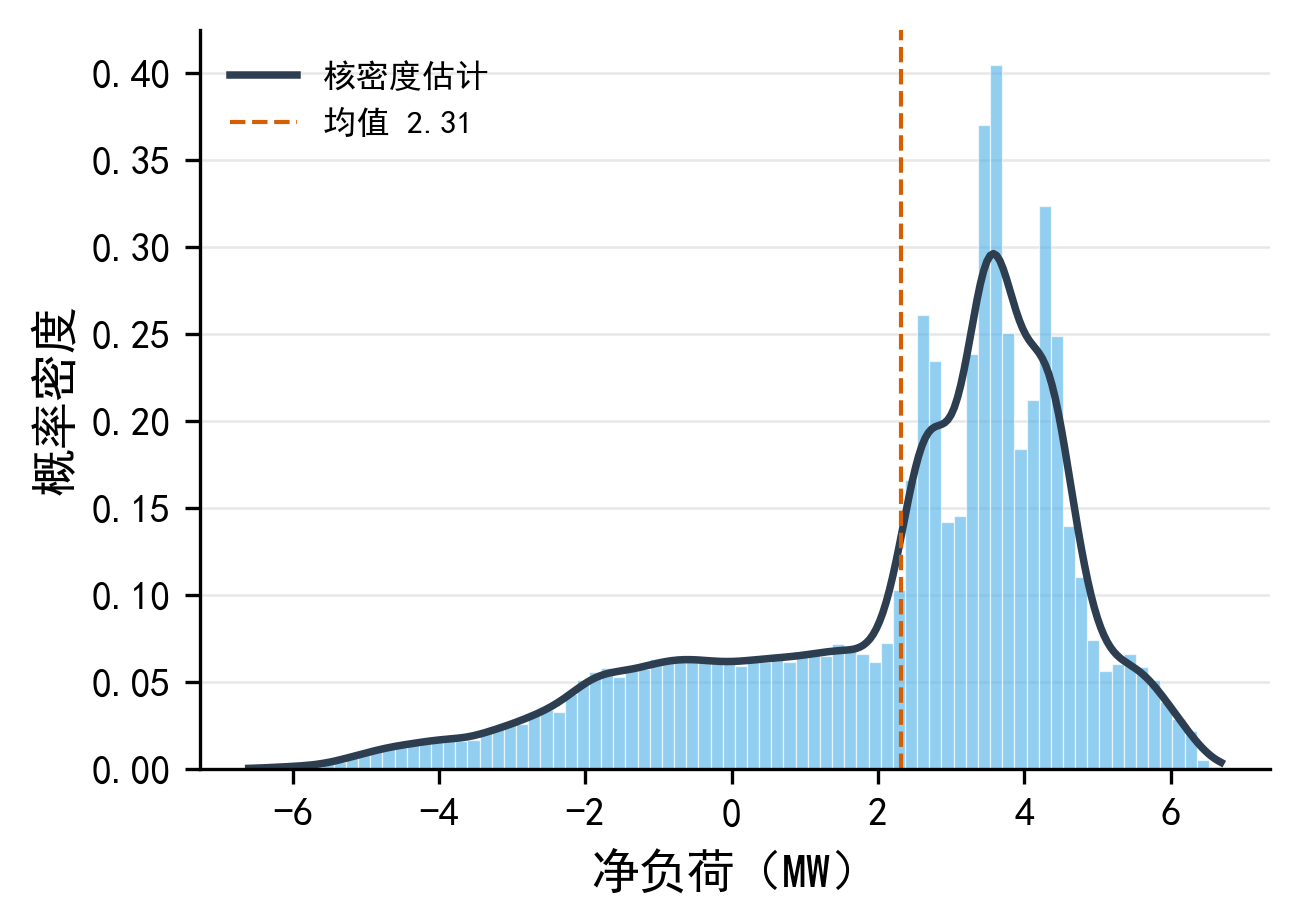
\includegraphics[width=0.75\textwidth]{figures/fig_eda_netload_dist.png}
  \caption{数据探索性分析：(a) 负载周几×时段热力图；(b) 光伏月度日发电量箱线图；(c) 固定与波动电价日内模式；(d) 全年净负荷分布}
  \label{fig:eda}
\end{figure}

\textbf{时段定义}。10 分钟粒度数据的行标签 $t$ 表示时段 $[t,\,t{+}10\,\mathrm{min})$ 的\textbf{起点}——依据是结果模板的时段标注（0:10--0:20、\ldots、0:00+1--0:10+1）与数据行标签一一对应。据此，一天 144 个时段构成计划窗口 $[0{:}10,\ \text{次日}0{:}10)$，其中 $[0{:}00,0{:}10)$ 归前一日计划覆盖。

\textbf{预报口径}。附件3 发布时刻 $T$ 的``预报$k$小时''经交叉验证确认为 $T{+}k$ \textbf{整点时刻的瞬时功率}：预报值与实际整点值的中位偏差仅 2.35 kW，48.5\% 的整点完全一致（非整点处的差异源于光伏出力的日内波动，而非预报口径错误）。由整点值线性插值得到 10 分钟粒度预测。

\textbf{数据质量}。全年 365 天 $\times$ 144 时段的负载、光伏与电价数据均无缺失值、无异常值（3$\sigma$ 检验通过），直接进入建模。

\section{模型假设}

\begin{enumerate}
  \item 赛题附件数据真实有效，10 分钟粒度的功率与电价为对应时段的平均值，全年数据无缺失；
  \item 微网不向外网售电（题目未提供上网机制），过剩电能只可充电或弃置；
  \item 光伏弃电自由且无成本；储能充电与放电功率上限 5000 kW 分别独立生效；
  \item 充放电效率 90\% 双向作用：并网侧充入 $c$ 电量使储电量增加 $0.9c$，并网侧放出 $d$ 电量使储电量减少 $d/0.9$；
  \item 计划购电量按计划量结算（take-or-pay），无论实际是否需要；实际供给不足负载部分按交易时刻电价的 5 倍紧急购电；
  \item 储能按日循环运行（0:00 与 24:00 储电量相同）：问题一为题设要求；问题二至四的\textbf{规划层}以日循环为终端目标（$s_{143} = s_0$），实际执行因预测误差可偏离该目标，跨日通过 SOC 连续传递保证系统可持续运行；
  \item 一天内储能设备参数恒定，外网供电可靠，紧急购电无容量限制。
\end{enumerate}

\section{符号说明}

\begin{table}[H]
  \centering
  \caption{主要符号与定义}
  \label{tab:symbols}
  \begin{tabularx}{0.88\textwidth}{C{0.14\textwidth}Y R}
    \toprule
    符号 & 含义 & 单位 \\
    \midrule
    $\Delta t$ & 时段长度，$\Delta t=1/6$ h & h \\
    $p_t$ & 时段 $t$ 电价 & 元/kWh \\
    $L_t,\ P_t$ & 时段 $t$ 小区负载、光伏功率 & kW \\
    $g_t$ & 时段 $t$ 计划购电量（并网侧） & kWh \\
    $a_t$ & 时段 $t$ 调整后购电量 & kWh \\
    $c_t,\ d_t$ & 时段 $t$ 储能充、放电量（并网侧） & kWh \\
    $v_t$ & 时段 $t$ 弃电量 & kWh \\
    $e_t$ & 时段 $t$ 紧急购电量 & kWh \\
    $s_t$ & 时段 $t$ 末储电量 & kWh \\
    $\eta$ & 充放电效率，$\eta=0.9$ & -- \\
    $\bar P$ & 最大充放电功率，$\bar P=5000$ & kW \\
    $\underline S,\ \overline S$ & 储电量下、上限（1200、10800） & kWh \\
    $\delta_t^{+},\ \delta_t^{-}$ & 时段 $t$ 购电量调增、调减量 & kWh \\
    \bottomrule
  \end{tabularx}
\end{table}

\section{问题一：确定性日循环购电模型的建立与求解}

\subsection{建模准备}

问题一中每天的电价与负载相同（附件1），光伏发电功率一天的预测数据给定，因而典型日的最优策略即每日重复的策略。该问为确定性资源调配问题，采用线性规划建模~\cite{jiang2003modeling}。将一天划分为 144 个 10 分钟时段，在钟表日 $[0{:}00,24{:}00)$ 上建立线性规划：时段 $j=0,1,\ldots,143$ 覆盖 $[j\Delta t,\,(j{+}1)\Delta t)$，其中 $[0{:}00,0{:}10)$ 时段的数据由附件1 末行（标签 0:00+1）给出——由于每天运行条件相同，该时段与次日首时段数据一致。附录1 给定 2025 年 1 月 1 日 0:00 储电量为 6000 kWh，取 $s_{-1}=6000$。

\subsection{模型建立}

决策变量为各时段购电量 $g_j$、充电量 $c_j$、放电量 $d_j$ 与弃电量 $v_j$。以全天购电费最小为目标：
\begin{equation}
  \min\ Z=\sum_{j=0}^{143} p_j\, g_j .
  \label{eq:q1obj}
\end{equation}

\textbf{（1）储能电量平衡}。充电经效率 $\eta$ 计入储能，放电按 $1/\eta$ 折减储能：
\begin{equation}
  s_j = s_{j-1} + \eta\, c_j - \frac{d_j}{\eta},\qquad j=0,1,\ldots,143;\qquad s_{-1}=6000 .
  \label{eq:q1soc}
\end{equation}

\textbf{（2）充放电功率与电量约束}：
\begin{equation}
  0\le c_j\le \bar P\Delta t,\qquad 0\le d_j\le \bar P\Delta t,\qquad
  \underline S\le s_j\le \overline S .
  \label{eq:q1power}
\end{equation}

\textbf{（3）供需平衡}。微网供电不得低于负载，购电、光伏与放电之和等于负载、充电与弃电之和：
\begin{equation}
  g_j + P_j\Delta t + d_j = L_j\Delta t + c_j + v_j,\qquad g_j,\,v_j\ge 0 .
  \label{eq:q1balance}
\end{equation}

\textbf{（4）日循环约束}。储能 0:00 与 24:00 储电量相同：
\begin{equation}
  s_{143} = 6000 .
  \label{eq:q1cycle}
\end{equation}

模型 \eqref{eq:q1obj}--\eqref{eq:q1cycle} 为线性规划。在当前假设下（电价恒正、光伏可免费弃电），可证存在不含同时充放电的不劣解：设某时段 $c_j, d_j > 0$，取 $\alpha = \min(c_j,\, d_j/\eta^2)$，令 $c_j' = c_j - \alpha$、$d_j' = d_j - \eta^2\alpha$，则 SOC 变化量不变，且 $c_j' + d_j' < c_j + d_j$，释放的能量可减少购电或增加弃电，总费用不增。求解时对充放吞吐加微罚（$10^{-7}$ 元/kWh）辅助选解；经验证全部结果中同时充放电时段数为 0，无需引入 0--1 互斥变量。

\subsection{求解方法}

模型含 865 个决策变量、289 个等式约束，采用 Python 的 SciPy~\cite{virtanen2020scipy} 接口调用 HiGHS 对偶单纯形求解器~\cite{huangfu2018highs}直接求解，单次求解耗时约 0.1 秒，得到全局最优解。求解后逐时段校验荷电状态区间、功率上限、能量平衡与循环条件，全部以 $10^{-4}$ 容差通过。

\subsection{结果与分析}

最优策略下全天购电量 59482.70 kWh，购电费 \textbf{35126.85 元}。表~\ref{tab:q1buy} 与表~\ref{tab:q1cd} 按题目要求格式给出指定时段结果，完整结果见支撑材料 \texttt{result1.xlsx}。

\begin{table}[H]
  \centering
  \caption{微网在指定时间段的购电量及全天的购电量和购电费}
  \label{tab:q1buy}
  \begin{tabularx}{0.92\textwidth}{C{0.18\textwidth} R C{0.18\textwidth} R C{0.18\textwidth} R}
    \toprule
    时间段 & 购电量/kWh & 时间段 & 购电量/kWh & 时间段 & 购电量/kWh \\
    \midrule
    10:00--10:10 & 0.00 & 12:00--12:10 & 486.40 & 14:00--14:10 & 0.00 \\
    16:00--16:10 & 394.93 & 18:00--18:10 & 636.98 & 20:00--20:10 & 0.00 \\
    \midrule
    \multicolumn{2}{c}{全天购电量/kWh} & \multicolumn{2}{c}{59482.70} & \multicolumn{2}{c}{全天购电费/元\ \ 35126.85} \\
    \bottomrule
  \end{tabularx}
\end{table}

\begin{table}[H]
  \centering
  \caption{储能设备在指定时间段的充放电量及 0:00 和 24:00 的储电量}
  \label{tab:q1cd}
  \begin{tabularx}{0.92\textwidth}{C{0.16\textwidth} R R C{0.16\textwidth} R R}
    \toprule
    时间段 & 充电量/kWh & 放电量/kWh & 时间段 & 充电量/kWh & 放电量/kWh \\
    \midrule
    0:00--4:00 & 4500.00 & 0.00 & 12:00--16:00 & 6119.37 & 91.10 \\
    4:00--8:00 & 833.33 & 5947.42 & 16:00--20:00 & 0.00 & 5068.69 \\
    8:00--12:00 & 3954.63 & 2121.42 & 20:00--24:00 & 5333.33 & 3571.31 \\
    \midrule
    \multicolumn{3}{c}{0:00 储电量/kWh\quad 6000.00} & \multicolumn{3}{c}{24:00 储电量/kWh\quad 6000.00} \\
    \bottomrule
  \end{tabularx}
\end{table}

图~\ref{fig:q1} 给出最优策略的时序结构。典型日电价呈``凌晨低谷（0--6 时均价 0.4355 元/kWh）—早高峰（8 时 1.1617 元/kWh）—午间小低谷（12 时 0.4432 元/kWh）—晚高峰（20 时 1.3482 元/kWh）''的形态，最优策略呈现清晰的套利结构：

\begin{itemize}
  \item \textbf{低谷充电}：凌晨 0--4 时与午间以低谷电价购电充电，其中 12:00--12:10 在午间小低谷直接购电 486.40 kWh；
  \item \textbf{双峰放电}：早高峰（4:00--8:00 放电 5947.42 kWh）与晚高峰（16:00--20:00 放电 5068.69 kWh）以储能放电替代高价购电，高价时段（10:00、14:00、20:00）购电量均为 0；
  \item \textbf{光伏消纳}：午间光伏过剩电力全部充入储能（12:00--16:00 充电 6119.37 kWh），典型日弃电量为 0；晚高峰储能耗尽后（18:00--18:10）才以 1.2313 元/kWh 补购 636.98 kWh。
\end{itemize}

\begin{figure}[H]
  \centering
  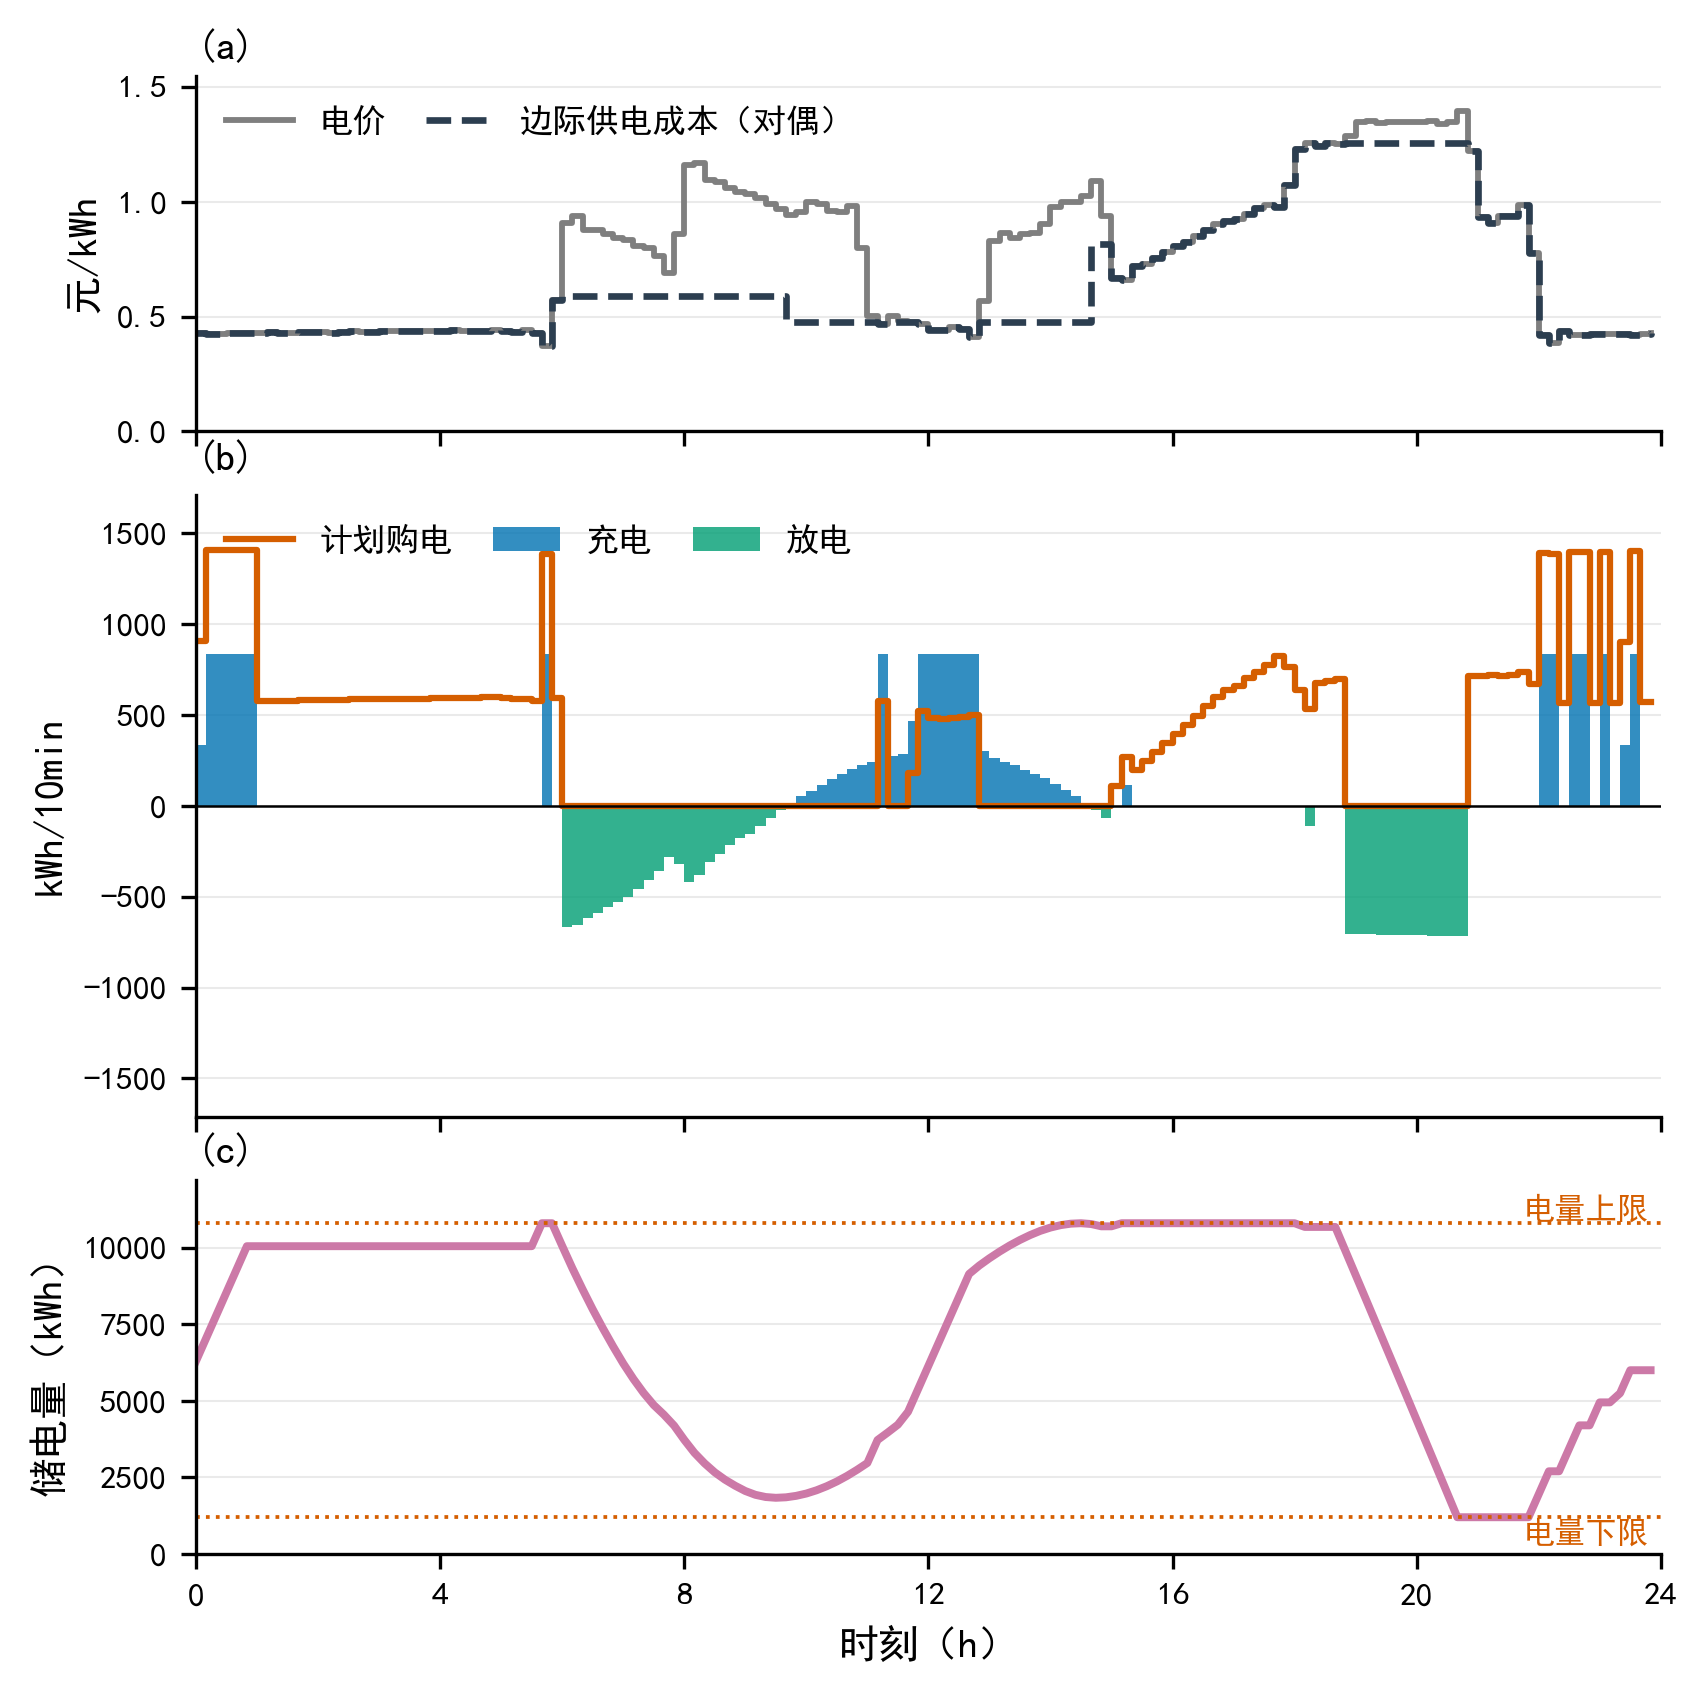
\includegraphics[width=0.95\textwidth]{figures/fig_q1_strategy.png}
  \caption{问题一最优策略与对偶分析：(a) 电价与边际供电成本（供需平衡约束的影子价格）；(b) 计划购电量与储能充放电；(c) 储电量轨迹}
  \label{fig:q1}
\end{figure}

与无储能基准（各时段购电量 $g_j=\max\{L_j\Delta t-P_j\Delta t,\,0\}$，购电费 48052.05 元）相比，储能调度使购电费降低 \textbf{12925.20 元（26.90\%）}。购电量本身亦由 61789.94 kWh 降至 59482.70 kWh：基准方案在午间弃置过剩光伏、晚间高价回购，储能一方面回收了这部分过剩光伏（净回收 2307.24 kWh），另一方面通过峰谷转移摊薄电价。

\textbf{对偶分析：边际供电成本}。模型 \eqref{eq:q1obj}--\eqref{eq:q1cycle} 供需平衡约束的影子价格即为各时段的\textbf{边际供电成本}——多供 1 kWh 负载所增加的最优费用，见图~\ref{fig:q1}(c)。其全天均值为 0.645 元/kWh，低于电价均值：在低谷与午间小低谷时段，边际供电成本与电价重合（直接购电）；在早晚高峰时段，储能放电将边际供电成本压至低于电价（最大 1.256 元/kWh 出现在储能耗尽的晚高峰末段），这正是套利收益的来源。此外，储电量上界约束在 15 个时段具有正影子价格（最大 0.2017 元/kWh），即在这些时段扩充储能容量可直接降低购电费，与后文灵敏度分析中容量上限的显著影响互相印证。

\textbf{日循环电量水平的稳健性}。将循环水平 $s_{-1}$ 在 $[1200,10800]$ kWh 内以 600 kWh 步长扫描，购电费在 35118.95--35186.81 元之间变化，最优水平 8400 kWh 仅比题给初值 6000 kWh 低 7.90 元，说明最优策略对储能初始电量水平不敏感，日循环设定不损失经济性。

% ============================================================
% 问题二至四：计算完成后填写
% ============================================================

\section{问题二：随机负载与光伏下的日前计划与实时执行模型}

\subsection{建模准备}

问题二中电价逐日相同（附件1），而负载与光伏逐日变化。决策者在每天 0:00 只能利用\textbf{此前的历史实际数据}制定当日计划；白天按 10 分钟粒度执行，购电量按计划量结算（take-or-pay），实际供给低于负载的部分按交易时刻电价的 5 倍紧急购电。储能电量跨日连续传递，1 月为初始化过渡期，2025.2.1--12.31（334 天）为正式回测期。

\subsection{负载与光伏预测模型}

对全天 144 个时段分别构造预测器，候选方法均严格只使用历史数据（walk-forward），精度对比见表~\ref{tab:q2fc}：

\begin{table}[H]
  \centering
  \caption{预测方法 walk-forward 精度对比（2025.2--12.31，单位 kW）}
  \label{tab:q2fc}
  \begin{tabularx}{0.92\textwidth}{L R R R}
    \toprule
    预测方法 & 负载 MAE & 光伏 MAE & 净负荷 MAE \\
    \midrule
    惰性法（前一日曲线） & 650.0 & 185.3 & 744.2 \\
    近 7 日均值 & 781.2 & 153.4 & 795.0 \\
    同星期近 4 周均值 & 188.9 & 251.7 & 370.0 \\
    指数加权混合（近期+同星期） & 299.7 & 232.9 & 412.8 \\
    加权混合 v1（负载同星期均值、光伏近 7 日均值） & 188.9 & 153.4 & 284.9 \\
    \textbf{加权混合 v2（负载同星期近 3 周加权、光伏近 7 日加权）} & \textbf{169.1} & \textbf{149.7} & \textbf{266.1} \\
    \bottomrule
  \end{tabularx}
\end{table}

数据分析表明负载存在很强的周周期：星期效应可解释负载总方差的 85.3\%，故负载采用同星期预测，并以近 3 周 3:2:1 线性加权处理季节漂移（1 月暖机期内各窗长 MAE 差 $<4$ kW 不敏感，取 3 周为钝感区间中值）；光伏出力由天气主导、无明显周效应，采用近 7 日加权均值。二者组合的加权混合 v2 将净负荷 MAE 降至 \textbf{266.1 kW}（较 v1 的 284.9 再降 6.6\%，配对 Wilcoxon $p<10^{-16}$），作为主预测器。冷启动（1 月 1 日无历史）以附件1 典型日曲线为先验。图~\ref{fig:val_fc} 展示三个不同星期类型样本日的预测与实际对比：工作日负载的``双峰''形态与周末的低负载特征均被准确捕捉；光伏预测在晴天准确度高，多云日存在偏差（这正是 SAA 场景法需要刻画的误差来源）。图~\ref{fig:val_resid} 的残差分析表明净负荷预测误差近似正态（$R^2=0.987$），轻微厚尾源于多云天的光伏骤降——报童缓冲的分位数方法与 SAA 的场景法均不依赖正态假设，可自然处理该厚尾特征。

\begin{figure}[H]
  \centering
  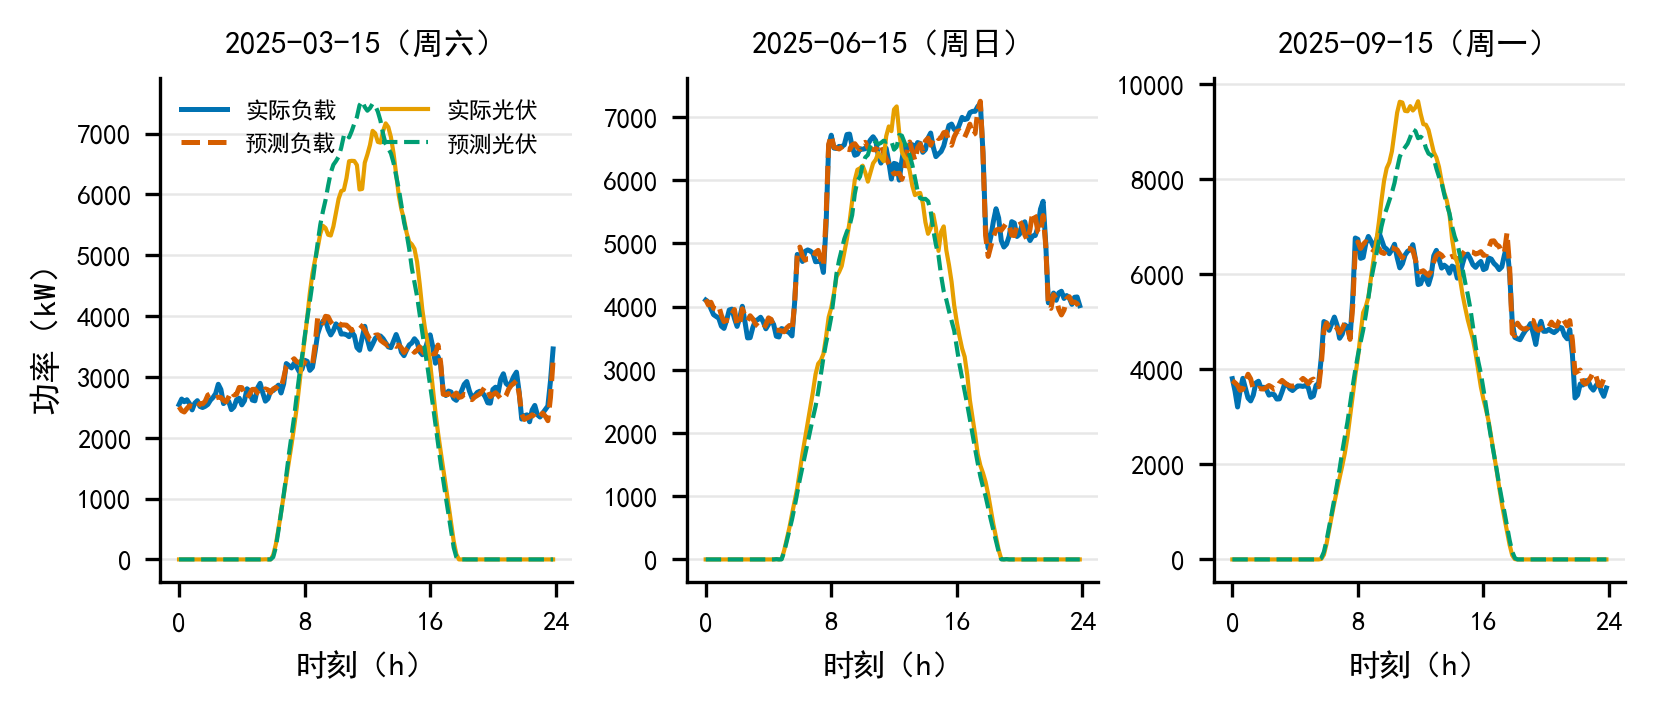
\includegraphics[width=0.95\textwidth]{figures/fig_val_forecast_overlay.png}
  \caption{预测与实际对比（三个样本日）：实线为实际值，虚线为预测值}
  \label{fig:val_fc}
\end{figure}

\begin{figure}[H]
  \centering
  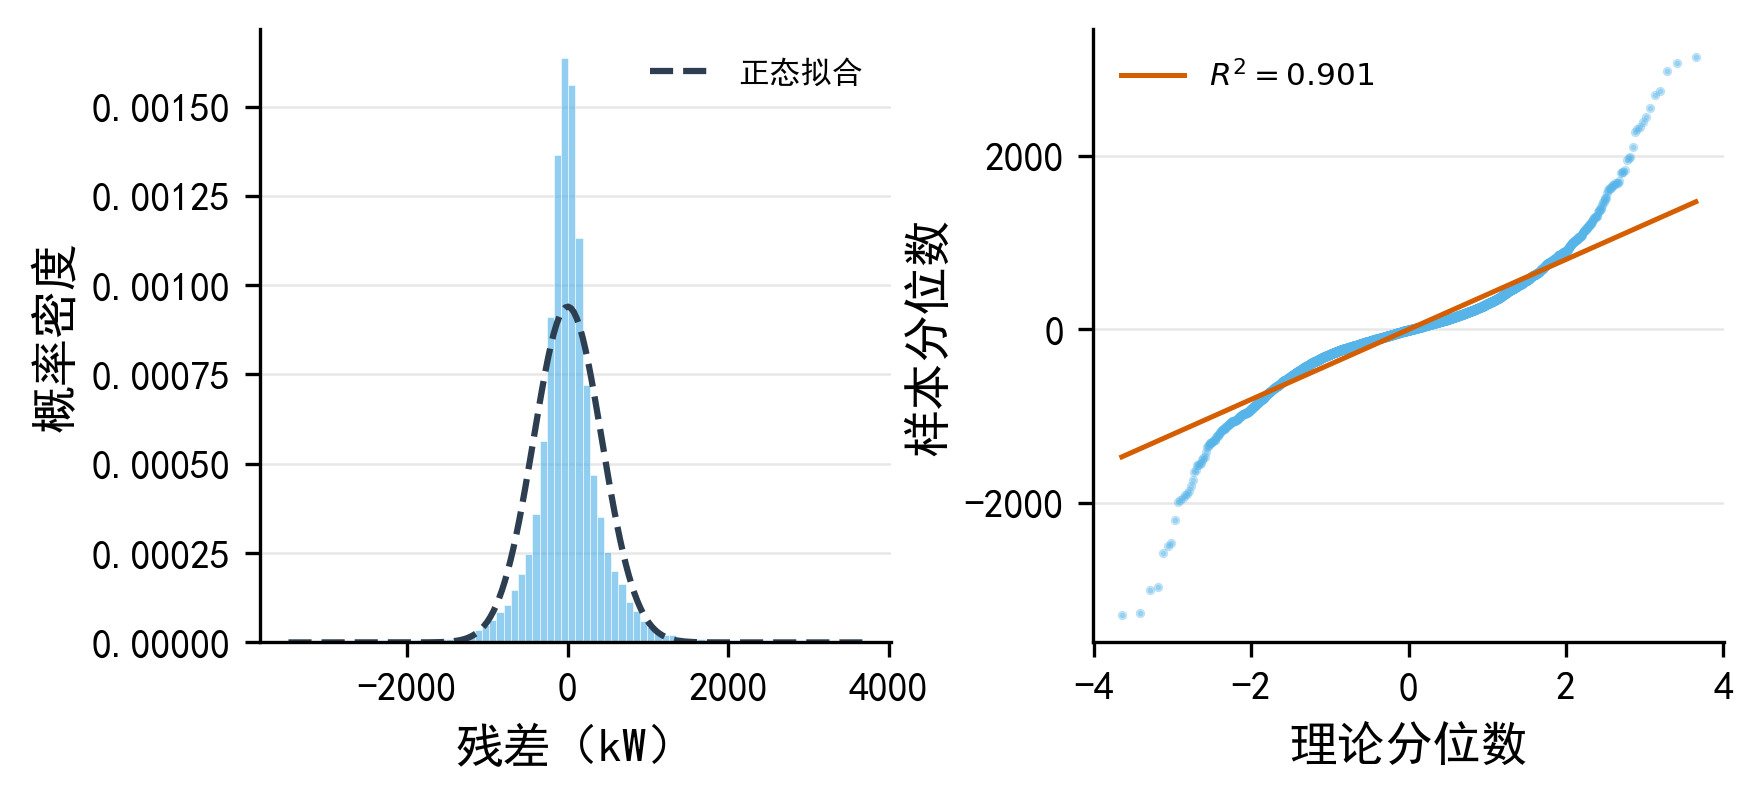
\includegraphics[width=0.92\textwidth]{figures/fig_val_residual.png}
  \caption{净负荷预测残差分析：(a) 残差直方图与正态拟合；(b) 正态 Q--Q 图}
  \label{fig:val_resid}
\end{figure}

\subsection{风险决策模型：报童缓冲与两阶段随机规划}

\subsubsection{报童缓冲——可解释的确定性等效方法}

计划购电量若仅按点预测制定，预测误差的右尾（实际净负荷高于预测）将触发 5 倍电价的紧急购电。设某时段净负荷 $n_t$ 的预测误差 $\varepsilon_t = n_t - \hat n_t$，计划量为 $\hat n_t + b_t$。每缺 1 kWh 需紧急购电多付 $5p_t - p_t = 4p_t$（相对按计划价购入），每多备 1 kWh 若无法利用则损失约 $p_t$（盈余可充电储存，损失折减）。由报童模型的一阶条件，最优准备量满足
\begin{equation}
  P\big(\varepsilon_t \le b_t^*\big) = \frac{4p_t}{4p_t + p_t} = 0.8,
  \label{eq:newsvendor}
\end{equation}
即取净负荷预测误差分布的 80\% 分位数（储能的残值效应使最优值略高）。该方法取近 28 天逐时段误差经验分位数 $b_t = \big[P_q(\varepsilon_t)\big]^+$ 抬升负载预测，概念清晰、计算极简，但其局限同样明显：逐时段独立决策，无法感知储能的跨时段耦合与计划量的整体最优性。

\subsubsection{两阶段随机规划——主模型}

为克服上述局限，本文进一步以近 $S$ 天的净负荷预测误差\textbf{整条曲线}为等概率经验场景，建立两阶段随机规划（SAA 近似）：第一阶段在 0:00 决策计划购电量 $g_t$（take-or-pay，各场景共用）；第二阶段在各场景 $s$ 下决策充电 $c_t^{(s)}$、放电 $d_t^{(s)}$、弃电 $v_t^{(s)}$、紧急购电 $e_t^{(s)}$ 及储能轨迹 $s_t^{(s)}$：
\begin{align}
  \min\ & \sum_{t=0}^{143} p_t g_t + \frac{1}{S}\sum_{s=1}^{S}\sum_{t=0}^{143} 5 p_t\, e_t^{(s)}
  \label{eq:saaobj}\\
  \text{s.t.}\quad
  & s_t^{(s)} = s_{t-1}^{(s)} + \eta c_t^{(s)} - d_t^{(s)}/\eta,\qquad s_{-1}^{(s)} = s_0,\quad s_{143}^{(s)} = s_0,
  \label{eq:saasoc}\\
  & g_t + d_t^{(s)} + e_t^{(s)} = \big(\hat n_t + \varepsilon_t^{(s)}\big)\Delta t + c_t^{(s)} + v_t^{(s)},
  \label{eq:saabal}\\
  & 0 \le c_t^{(s)}, d_t^{(s)} \le \bar P \Delta t,\quad \underline S \le s_t^{(s)} \le \overline S,\quad g_t, v_t^{(s)}, e_t^{(s)} \ge 0,
  \nonumber
\end{align}
其中 $\varepsilon_t^{(s)}$ 为场景 $s$（历史某日）的净负荷预测误差。模型以\textbf{期望总费用}为目标，将风险准备、储能时移与 take-or-pay 结算结构内生化：报童缓冲是其无储能、单时段的特例。场景数 $S$ 于 1 月（过渡期）在 $\{10,14,28\}$ 中以滚动总费用选定（分别为 207.2 / 212.9 / 214.0 万元，得 $S^*=10$，近因场景更具代表性）。单日模型含约 $1.6\times 10^4$ 个变量，HiGHS 求解约 0.5 秒，全年 365 天求解累计约 3 分钟。

\subsection{日前计划与实时执行}

\textbf{计划层}：主策略以两阶段随机规划 \eqref{eq:saaobj}--\eqref{eq:saabal} 求计划购电量 $g_t$（$s_0$ 为当日实际继承电量，日循环）；报童缓冲 + 问题一 LP 框架作为对照策略。

\textbf{执行层}：购电量按计划强制执行，储能实时调度。盈余（$g_t + P_t\Delta t > L_t\Delta t$）按上限充电、越限弃电——该规则恒为最优（盈余电能机会成本为零）；缺口时段存在``立即放电''与``保留电量规避未来更高价紧急购电''的权衡，本文比较两种策略：
\begin{itemize}
  \item \textbf{贪心执行}：缺口即放电至上限，不足部分紧急购电；
  \item \textbf{滚动执行}：缺口时对当日剩余时段重解一个小规模 LP（购电量锁定、当前时段用实际值、未来用当日预测、终端回到当日循环水平），据影子价格决定本时段放电量，将紧急购电转移到低价时段。
\end{itemize}

\textbf{超参数选择协议}：场景数 $S$ 与对照策略的缓冲分位数 $q$ 均在 1 月（过渡期）以滚动总费用选定（$S^*=10$；$q^*=0.7$，理论值 0.8 亦在平坦最优区内）；2--12 月为正式回测期，其费用仅用于报告与敏感性分析，不参与选择，杜绝信息泄露。

\subsection{结果与分析}

各策略在正式回测期的总费用见表~\ref{tab:q2cmp}，费用构成见图~\ref{fig:q2cmp}。

\begin{table}[H]
  \centering
  \caption{问题二各策略回测期总费用对比（2025.2.1--12.31）}
  \label{tab:q2cmp}
    \begin{tabularx}{0.94\textwidth}{L R R R}
    \toprule
    策略 & 总费用/元 & 其中紧急购电费/元 & 紧急占比 \\
    \midrule
    无储能基准 & 16,407,320 & 0 & 0.0\% \\
    朴素预测（无缓冲）+ 贪心执行 & 15,402,753 & 538,911\,$\times$\,5 & 17.5\% \\
    报童缓冲（$q{=}0.7$）+ 贪心执行 & 14,129,870 & 183,652\,$\times$\,5 & 13.0\% \\
    报童缓冲（$q{=}0.7$）+ 滚动执行 & 14,039,965 & 936,376 & 6.7\% \\
    单侧保守化分位数等效 + 滚动执行 & 14,574,928 & 1,690,964 & 11.6\% \\
    CVaR-SAA（$\alpha{=}0.95,\lambda{=}0.1$）+ 滚动执行 & 13,886,358 & 1,032,418 & 7.4\% \\
    SAA + 全时域 MPC 执行 & 15,370,671 & 2,559,614 & 16.7\% \\
    \textbf{两阶段随机规划（$S{=}10$）+ 滚动执行（主策略）} & \textbf{13,879,046} & \textbf{1,028,406} & \textbf{7.4\%} \\
    理想先知（完全预测基准） & 12,245,047 & 0 & 0.0\% \\
    \bottomrule
  \end{tabularx}
\end{table}

主策略较无储能基准节省 \textbf{2,528,274 元（15.41\%）}，较朴素预测策略节省 \textbf{1,523,707 元（9.89\%）}，距理想先知基准 13.34\%。各策略的边际贡献如下：

\textbf{（1）报童缓冲的价值}：使紧急购电费从 538,911$\times$5 元（朴素贪心）降至 936,376 元（滚动执行），体现式~\eqref{eq:newsvendor} 的风险对冲作用。

\textbf{（2）滚动执行的价值}：将紧急购电从贪心放电改为按剩余日电价结构优化放电时机——紧急电量从贪心的 183,652 kWh 略增至 209,621 kWh，但平均结算价从 6.04 降至 4.47 元/kWh，总费用降低 9 万元。

\textbf{（3）两阶段随机规划的价值}：在报童缓冲之上再节省 \textbf{160,919 元}——分位数缓冲逐时段独立决策导致\textbf{过度防御}（多购的计划电量在多数日被弃置），SAA 在期望意义下取得全局精确平衡。

\textbf{（4）加权混合 v2 预测器的价值}：净负荷 MAE 从 284.9 降至 266.1 kW（$p<10^{-16}$），额外贡献 5.9 万元。

\textbf{证伪实验}。本文系统测试了九种替代方案（表~\ref{tab:q2cmp} 中列 CVaR-SAA 与全时域 MPC 两行，另有 E1--E7 见代码文档），均未超过主策略。两项最具代表性的证伪如下：

\textbf{（a）CVaR-SAA 证伪}：在期望费用上叠加条件风险价值（$\alpha\in\{0.90,0.95\}$、$\lambda\in\{0.1,0.3,0.5\}$ 全网格），任何正的 $\lambda$ 均劣于纯期望最优——5 倍紧急购电价\textbf{本身已内嵌足够强的风险惩罚}，再叠加 CVaR 导致双重风险规避与过度保守。

\textbf{（b）全时域 MPC 证伪}：每 10 分钟对剩余日重解 LP（而非仅在缺口时干预），总费用反升 10.75\%——频繁用不完美预测重优化\textbf{损害了} SAA 计划的全局最优性。

这九组对照共同表明：\textbf{``SAA 期望最优 + 缺口时滚动干预''取得了最低回测费用}——过度建模（CVaR）与过度控制（MPC）均适得其反。全年 334 天中 218 天发生紧急购电，但紧急电量仅占购电量的 1.0\%。

图~\ref{fig:val_soc} 展示主策略的全年储电量轨迹：储电量长期维持在 8000--10800 kWh 区间（受上界约束），偶有工作日午后放电至 4000--6000 kWh 后迅速回充，日循环约束得到严格满足。图~\ref{fig:val_cost} 的月度费用分解显示：计划购电费全年均匀分布（约 100 万元/月），而紧急购电费集中在夏季（6--8 月，月均 15--20 万元）——夏季多云天气导致光伏预测误差增大，触发更多紧急购电。

\begin{figure}[H]
  \centering
  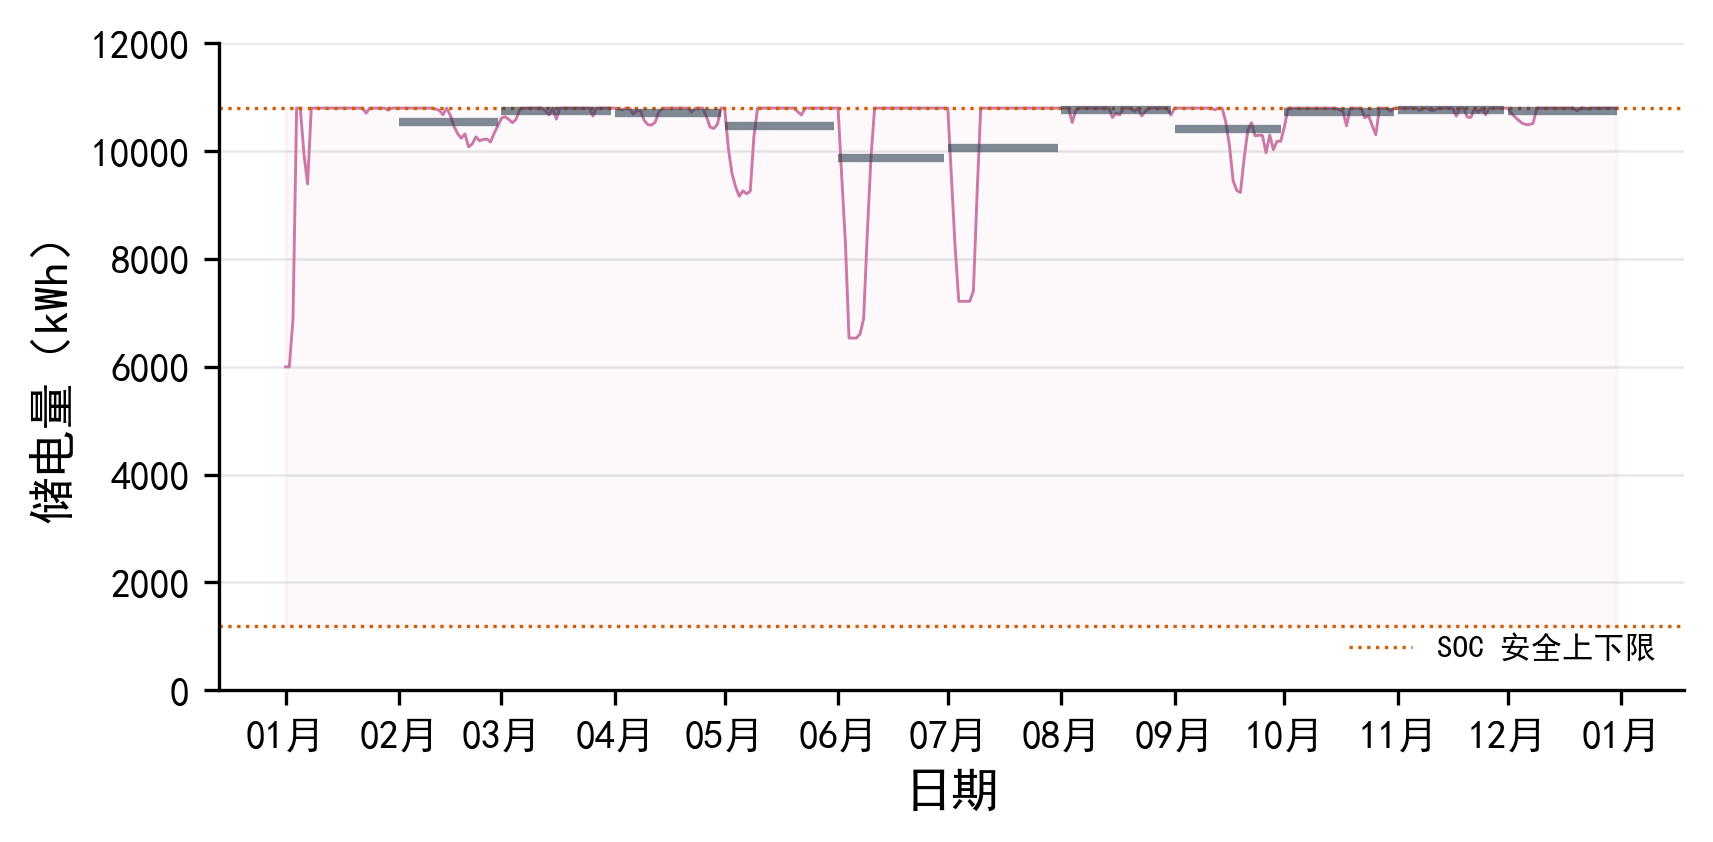
\includegraphics[width=0.95\textwidth]{figures/fig_val_soc_year.png}
  \caption{主策略全年储电量轨迹（粗线为月均值）}
  \label{fig:val_soc}
\end{figure}

\begin{figure}[H]
  \centering
  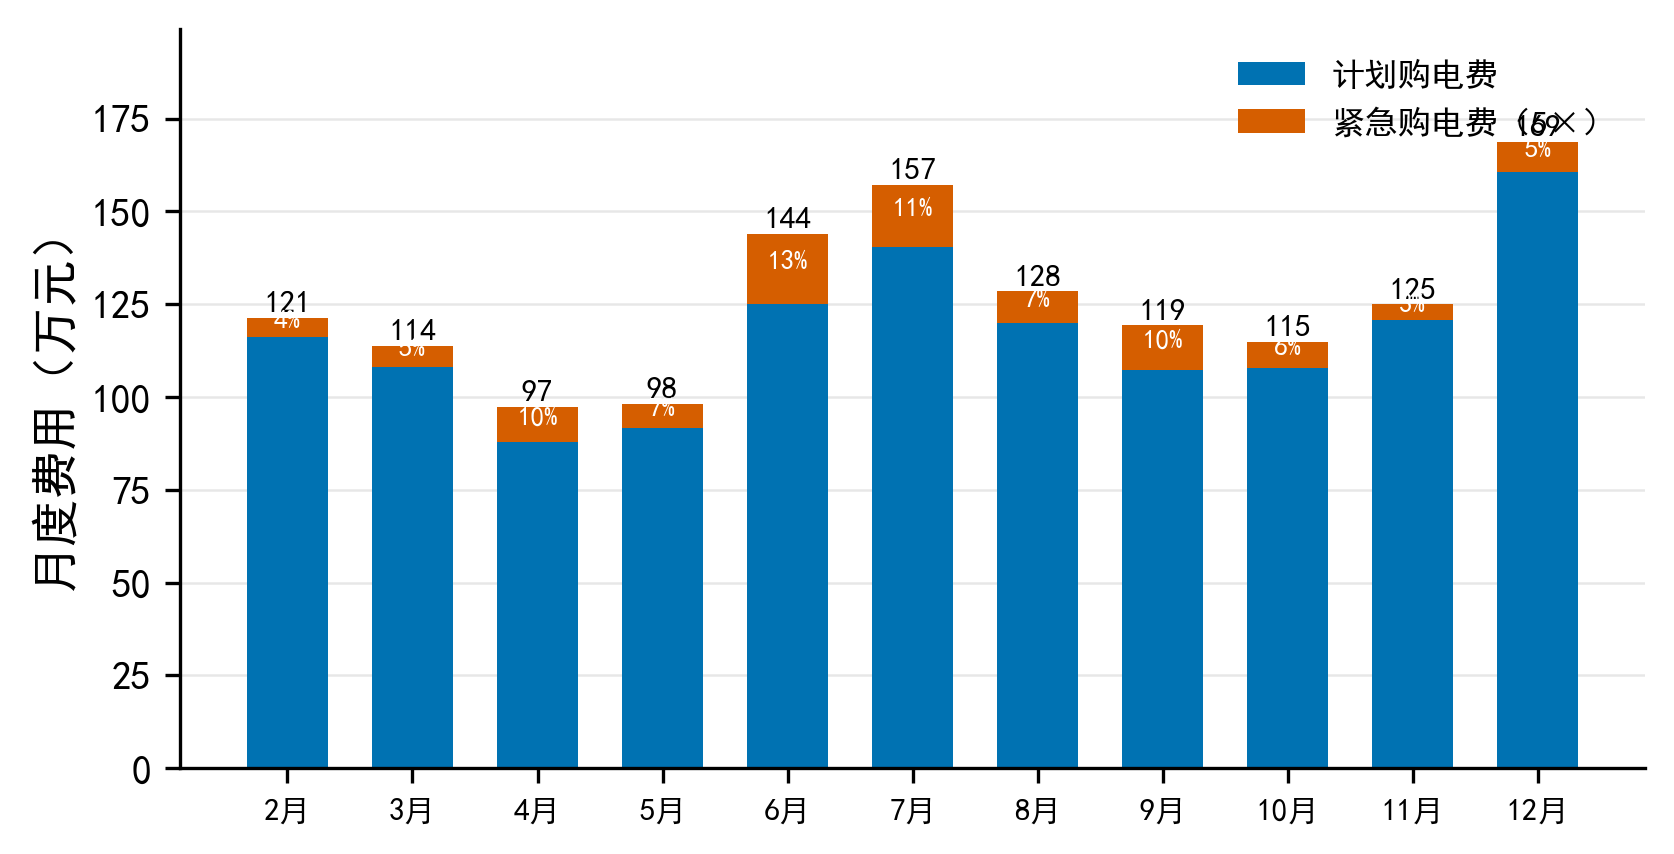
\includegraphics[width=0.92\textwidth]{figures/fig_val_monthly_cost.png}
  \caption{主策略月度费用分解：计划购电费与紧急购电费（2025.2--12 月）}
  \label{fig:val_cost}
\end{figure}

\textbf{信息价值分解与信息结构敏感性}。将信息条件逐级放松可定位改进空间：完美预见（负载与光伏均已知）为 12,245,047 元；负载已知、光伏按预测（仍用两阶段随机规划）为 \textbf{13,035,605 元}；双侧均按预测（主策略，严格遵循题目``每天 0:00 制定当天计划''的信息结构）为 \textbf{13,879,046 元}。

该分解的第二档位具有直接的跨方法比较意义：若采用``附件2 当日数据可直接作为日前计划输入''的解读（即假设负载日前完全已知），本文的两阶段随机规划达到 13,035,605 元，优于该信息结构下的保守分位数等效方法（13,200,522 元）与全部基于确定性缓冲的方案——即本文优化框架在更强信息假设下同样保持最优性。而主结果采用双侧预测口径，是因为``0:00 制定当天计划''意味着当日负载不可预知，该口径才是符合题意的信息结构。据此，距完美预见的总差距 1,633,999 元中，\textbf{光伏不确定性贡献 790,558 元（48.4\%），负载预测误差贡献 843,441 元（51.6\%）}——两侧几乎各半，表明进一步压缩总费用的空间主要在预测精度而非决策机制；且即便负载完全已知，仅光伏不确定性仍造成 6.5\% 的费用损失，从信息上限角度印证了本文决策机制已接近该信息结构下的最优。

图~\ref{fig:q2sens} 给出对照策略的缓冲分位数敏感性：总费用在 $q \in [0.7, 0.8]$ 内处于平坦最优区（14.04 百万元），偏离该区间后费用上升；理论值 0.8 与调参值 0.7 均落在平坦区内，说明报童理论的正确性与结论的稳健性。

\begin{figure}[H]
  \centering
  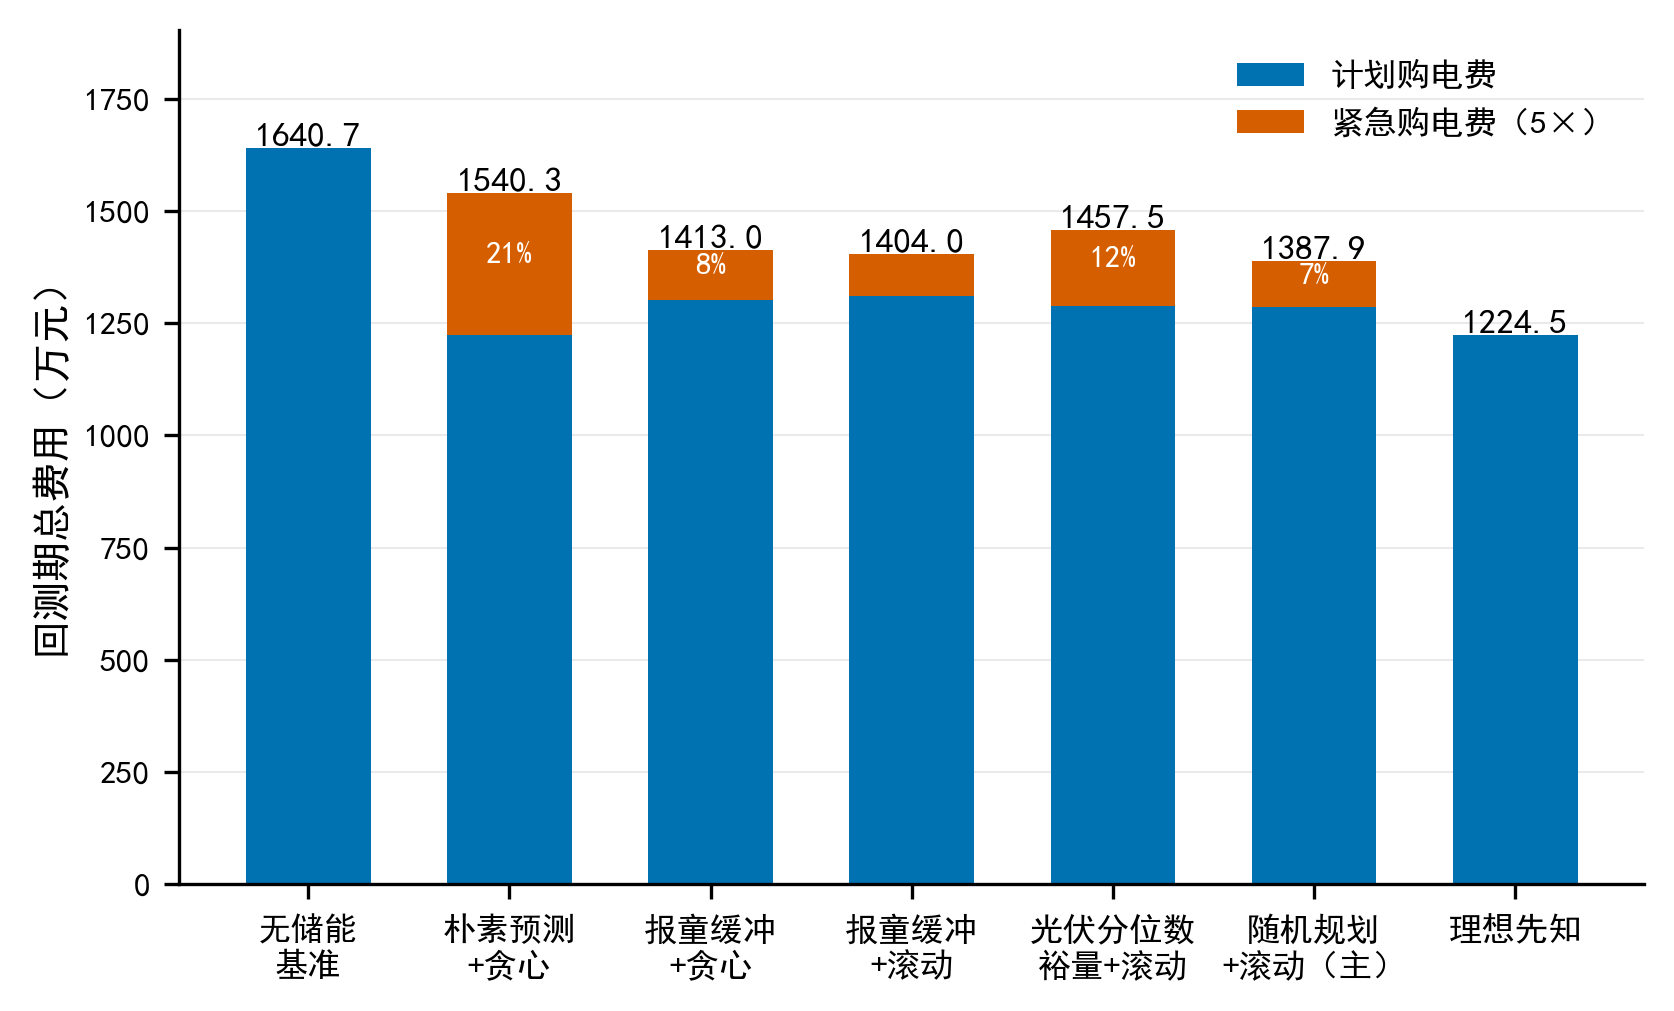
\includegraphics[width=0.8\textwidth]{figures/fig_q2_strategy_cmp.png}
  \caption{问题二各策略全年购电费用对比}
  \label{fig:q2cmp}
\end{figure}

\begin{figure}[H]
  \centering
  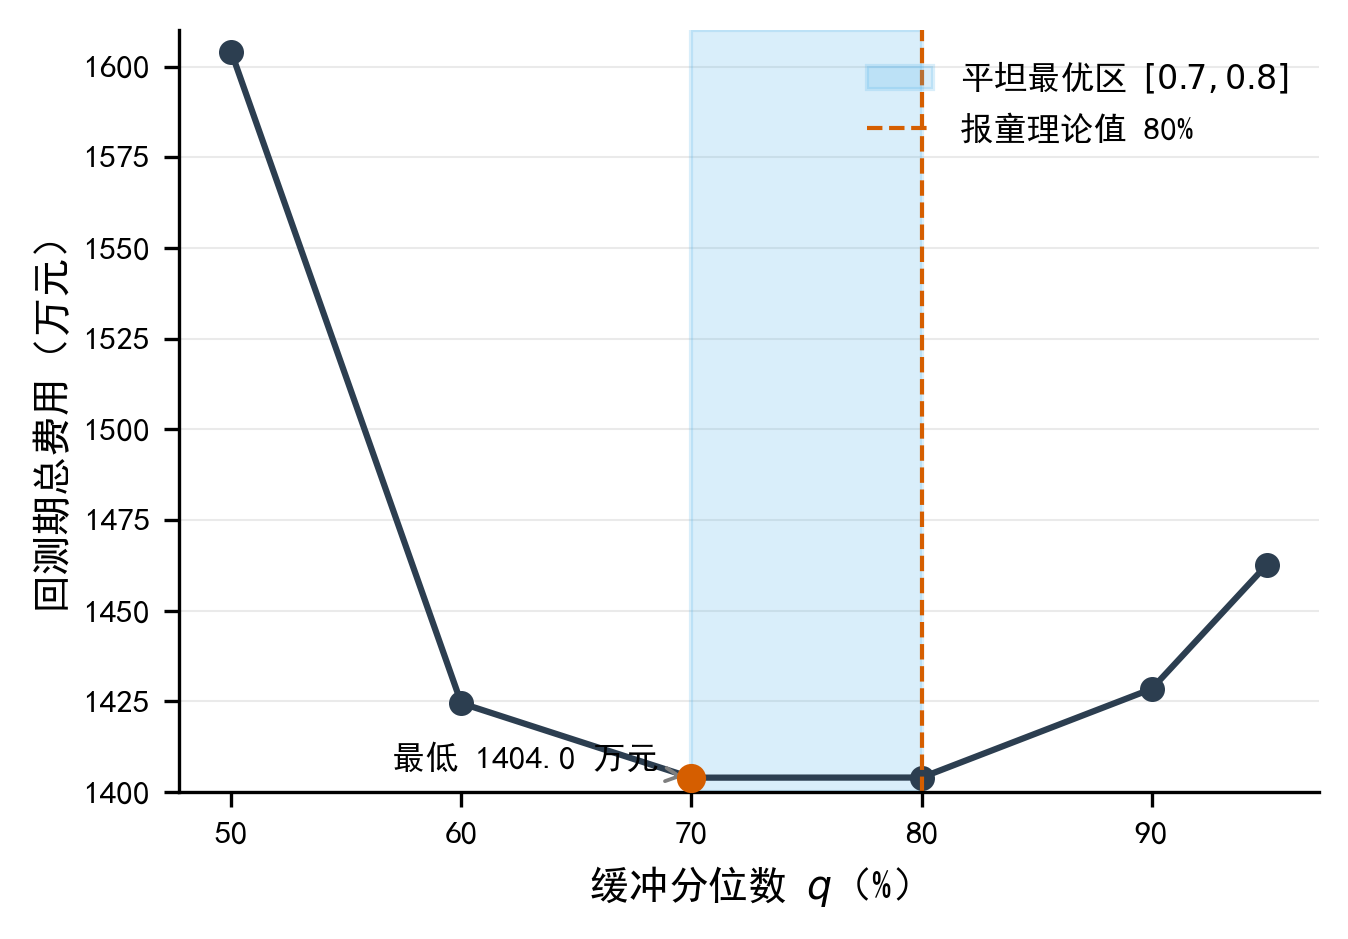
\includegraphics[width=0.62\textwidth]{figures/fig_q2_sens_q.png}
  \caption{缓冲分位数敏感性（滚动执行）}
  \label{fig:q2sens}
\end{figure}

题目指定日期的结果见表~\ref{tab:q2dates1}--\ref{tab:q2emg}。四个日期分别代表春季平常日（3.20）、夏季光伏富余日（6.21，计划购电量仅 36,930.13 kWh，日初与日末储电量均达到上限 10800 kWh）、秋季预测误差最大日（9.23，紧急购电费 9,838.99 元）与冬季光伏匮乏日（12.21，计划购电量高达 95,961.96 kWh）。6.21 无紧急购电、12.21 仅 40.69 元，说明风险决策成功覆盖了这两日的预测误差。

\begin{table}[H]
  \centering
  \caption{指定日期的购电量（按表1格式，单位 kWh）}
  \label{tab:q2dates1}
  \begin{tabularx}{0.94\textwidth}{C{0.16\textwidth} R R R R}
    \toprule
    时间段 & 2025.3.20 & 2025.6.21 & 2025.9.23 & 2025.12.21 \\
    \midrule
    10:00--10:10 & 0.00 & 0.00 & 0.00 & 0.00 \\
    12:00--12:10 & 582.87 & 0.00 & 463.59 & 920.78 \\
    14:00--14:10 & 0.00 & 0.00 & 0.00 & 0.00 \\
    16:00--16:10 & 440.95 & 123.12 & 456.45 & 785.11 \\
    18:00--18:10 & 719.27 & 411.22 & 756.20 & 700.95 \\
    20:00--20:10 & 0.00 & 0.00 & 18.41 & 0.00 \\
    \midrule
    全天购电量 & 67,118.76 & 36,930.13 & 63,893.96 & 95,961.96 \\
    全天计划购电费/元 & 40,803.85 & 21,180.92 & 39,838.18 & 61,635.40 \\
    紧急购电费/元 & 1,819.49 & 0.00 & 9,838.99 & 40.69 \\
    \bottomrule
  \end{tabularx}
\end{table}

\begin{table}[H]
  \centering\footnotesize\setlength{\tabcolsep}{3pt}
  \caption{指定日期的储能充放电量与储电量（按表2格式，单位 kWh）}
  \label{tab:q2dates2}
  \begin{tabularx}{0.98\textwidth}{C{0.115\textwidth} R R R R R R R R}
    \toprule
    & \multicolumn{2}{c}{2025.3.20} & \multicolumn{2}{c}{2025.6.21} & \multicolumn{2}{c}{2025.9.23} & \multicolumn{2}{c}{2025.12.21} \\
    \cmidrule(lr){2-3}\cmidrule(lr){4-5}\cmidrule(lr){6-7}\cmidrule(lr){8-9}
    时间段 & 充电 & 放电 & 充电 & 放电 & 充电 & 放电 & 充电 & 放电 \\
    \midrule
    0:00--4:00 & 324.60 & 10.56 & 186.35 & 3155.96 & 950.33 & 222.10 & 947.17 & 390.91 \\
    4:00--8:00 & 269.60 & 4595.93 & 203.19 & 5387.84 & 657.78 & 5418.79 & 1213.85 & 759.18 \\
    8:00--12:00 & 4957.72 & 3265.56 & 10134.27 & 0.00 & 3391.21 & 2387.94 & 4747.90 & 7825.55 \\
    12:00--16:00 & 4794.69 & 346.39 & 24.08 & 0.00 & 6577.67 & 403.62 & 7696.48 & 2254.40 \\
    16:00--20:00 & 125.10 & 4982.33 & 76.78 & 4772.97 & 9.09 & 4762.98 & 35.86 & 4991.29 \\
    20:00--24:00 & 9899.88 & 3725.63 & 9589.62 & 3056.81 & 9160.25 & 3884.39 & 9975.24 & 3632.07 \\
    \midrule
    0:00 / 24:00 储电量 & \multicolumn{2}{c}{10519.59 / 10046.91} & \multicolumn{2}{c}{10800.00 / 10800.00} & \multicolumn{2}{c}{9750.12 / 9444.23} & \multicolumn{2}{c}{10132.97 / 10228.47} \\
    \bottomrule
  \end{tabularx}
\end{table}

\begin{table}[H]
  \centering
  \caption{指定日期的紧急购电量（按表3格式，单位 kWh）}
  \label{tab:q2emg}
  \begin{tabularx}{0.8\textwidth}{C{0.2\textwidth} C{0.28\textwidth} R}
    \toprule
    日期 & 紧急购电时间段 & 紧急购电量 \\
    \midrule
    2025.3.20 & 0:30--0:40 & 12.67 \\
     & 1:00--2:20 & 218.52 \\
     & 2:40--3:00 & 56.24 \\
     & 3:10--4:10 & 245.37 \\
     & 5:50--6:00 & 1.27 \\
     & 16:10--16:50 & 101.83 \\
     & 20:20--20:30 & 15.68 \\
     & 21:40--22:00 & 29.97 \\
    \midrule
    2025.6.21 & \multicolumn{2}{c}{无紧急购电} \\
    \midrule
    2025.9.23 & 0:10--0:20 & 4.74 \\
     & 0:40--1:40 & 250.32 \\
     & 2:10--2:20 & 76.97 \\
     & 15:00--15:30 & 644.69 \\
     & 16:00--18:00 & 626.63 \\
     & 18:10--19:00 & 289.27 \\
     & 20:20--20:40 & 87.68 \\
     & 21:00--22:00 & 388.57 \\
    \midrule
    2025.12.21 & 20:20--20:30 & 6.07 \\
    \bottomrule
  \end{tabularx}
\end{table}

紧急购电集中在两类时段（表~\ref{tab:q2emg}）：一是\textbf{凌晨}（0:00--4:00）——该时段无光伏，缺口完全由负载预测误差引起，且夜间电价低、滚动执行优先保留储电量应对日间高价，故小额缺口以紧急购电吸收更为经济；二是\textbf{午后至傍晚}（如 9.23 的 15:00--19:00）——多云天气下光伏实际出力低于预测且负载处于高位，储电量快速释放仍不足以覆盖。图~\ref{fig:q2day} 展示了正式期内紧急购电最严重日的调度细节。

\begin{figure}[H]
  \centering
  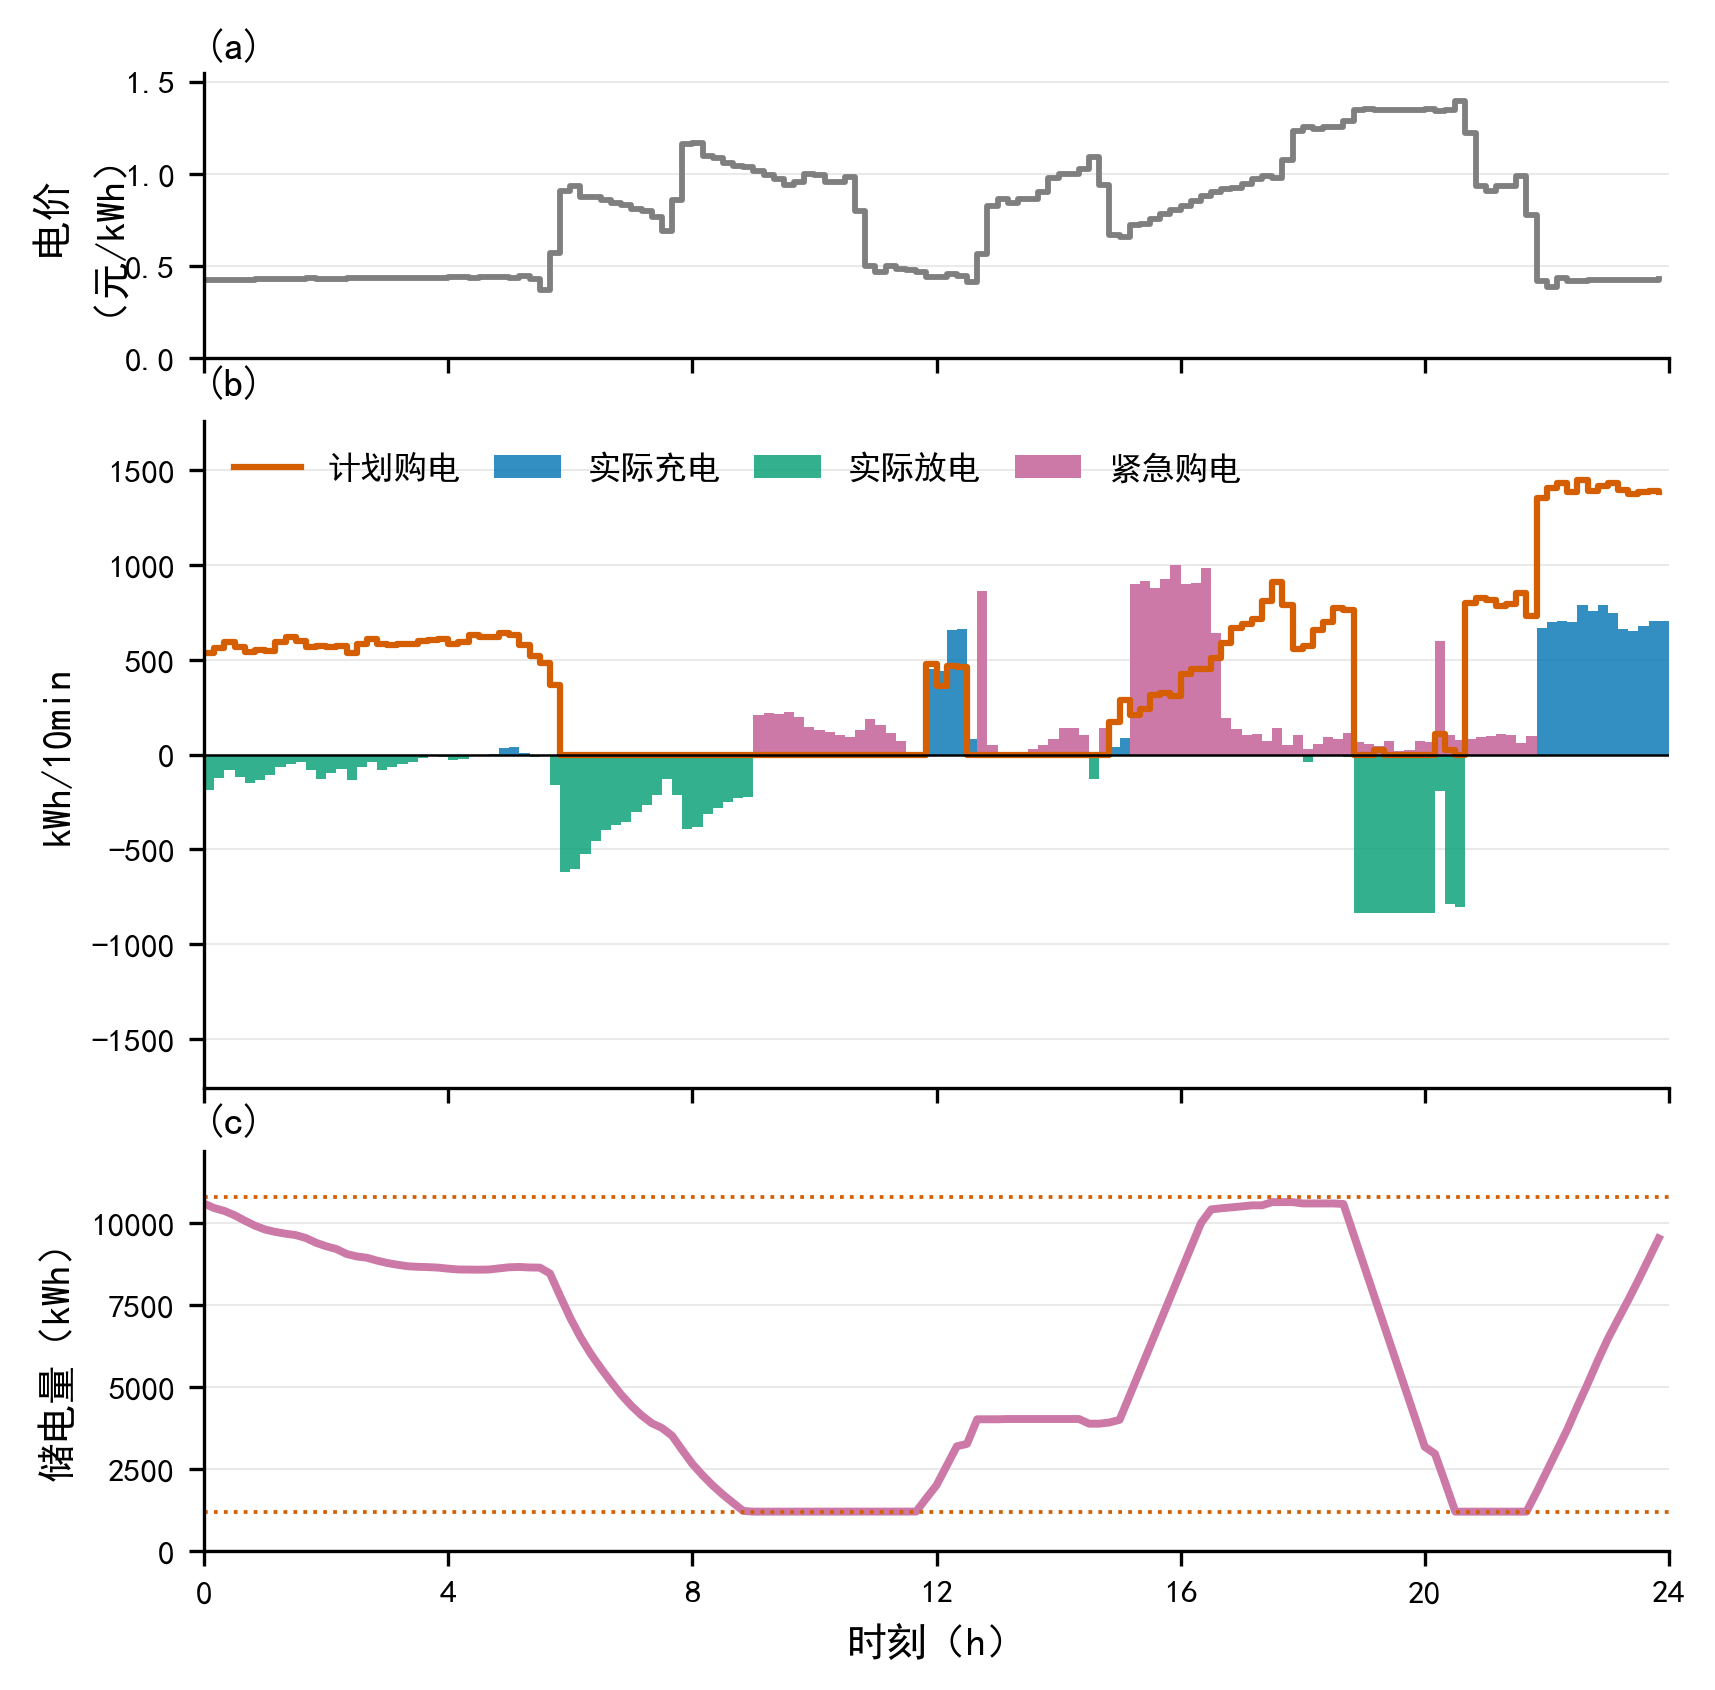
\includegraphics[width=0.95\textwidth]{figures/fig_q2_worst_day.png}
  \caption{主策略在紧急购电最严重日（2025.6.1）的调度：(a) 电价；(b) 计划购电、实际充放电与紧急购电；(c) 储电量轨迹}
  \label{fig:q2day}
\end{figure}

完整结果见支撑材料 \texttt{result2.xlsx}（334 天逐时段计划购电量、充放电量与紧急购电记录）。

\section{问题三：基于多时点预报的滚动调整购电模型}

\subsection{建模准备与信息分析}

问题三在问题二的基础上引入每天 0/6/12/18 时发布的光伏预报（附件3，每次覆盖未来 24 个整点），并允许根据新预报调整购电策略：调减部分按交易时刻电价的 50\% 结算（违约价），调增超出部分按 1.5 倍结算，紧急购电仍为 5 倍。

首先分析官方预报的信息价值。经验证，发布时刻 $T$ 的``预报$k$小时''即 $T{+}k$ 整点的瞬时功率（整点处中位偏差仅 2.35 kW），将其线性插值到 10 分钟槽后，0:00 发布预报的 MAE 为 197.5 kW，反而高于近 7 日历史均值的 153.4 kW——官方预报含显著噪声。而二者误差来源不同（预报噪声 vs.\ 气候均值的形状偏差），按按历史均方误差倒数加权组合可显著提升精度：逐槽以近 28 天两类预测的误差方差确定权重 $w_t = \sigma_{\mathrm{mean7},t}^2 / (\sigma_{\mathrm{fc},t}^2 + \sigma_{\mathrm{mean7},t}^2)$，组合预测 MAE 降至 \textbf{127.8 kW}。各发布时刻的组合精度为：0 时 127.8、6 时 132.2、12 时 58.1 kW（越临近越准）；18 时预报对当日调整\textbf{无信息价值}——19 时后光伏全年为零，其覆盖时段误差恒为 0。

\subsection{模型建立}

\textbf{计划层（0:00）}：与问题二主策略相同，采用两阶段随机规划 \eqref{eq:saaobj}--\eqref{eq:saabal}，其中光伏预测取``官方 0:00 预报 × 历史均值''的按均方误差倒数加权组合，负载预测同问题二，解得计划购电量 $g_t$。

\textbf{调整层（6/12/18 时发布，$T{+}1$ 时起执行）}：发布时刻 $T$ 的预报首个覆盖整点为 $T{+}1$ 时，故调整量从 $T{+}1$ 时起生效（$k \ge k_0(T)$：6 时对应 $k_0=41$，12 时 $k_0=77$，18 时 $k_0=113$）；$[T, T{+}1)$ 时段维持原计划不变。调整 LP 使用\textbf{$T{+}1$ 时（而非 $T$ 时）的实际储电量}作为初始状态——这是保守选择：$T$ 至 $T{+}1$ 的一小时执行结果已包含在初始 SOC 中，不引入额外预测误差，但与``$T$ 时即决策''的表述存在一小时时间差。
\begin{equation}
  a_k = g_k + \delta_k^+ - \delta_k^-, \qquad \delta_k^\pm \ge 0,\ k \ge k_0(T),
  \label{eq:q3dev}
\end{equation}
第二阶段以近 10 天\textbf{该发布时刻}新预报的净负荷误差 $\varepsilon_k^{(s)}$ 为等概率场景，决策各场景的充、放、弃、紧急购电：
\begin{equation}
  \min\ \sum_{k \ge k_0} \Big[ p_k a_k + 0.5\,p_k\big(\delta_k^+ + \delta_k^-\big) \Big]
  + \frac{1}{S}\sum_{s=1}^{S}\sum_{k \ge k_0} 5\,p_k\, e_k^{(s)},
  \label{eq:q3obj}
\end{equation}
约束与 \eqref{eq:saasoc}--\eqref{eq:saabal} 结构相同（自当前实际电量起、各场景日循环，供需平衡中的净负荷取新预报 $\hat n_k^{\mathrm{new}} - \varepsilon_k^{(s)}$）。式 \eqref{eq:q3obj} 中调减量系数 $0.5p_k$ 即``违约部分按 50\% 结算''，与调增超出部分的 1.5 倍（基准价之上加 $0.5p_k$）在结算结构上对称。值得强调的是，若调整层沿用确定性等效（点预测加报童缓冲）而计划层用随机规划，两层风险视角不一致会使调整反而受损——本文实验中，在该不一致设置下单独引入 6/12/18 时调整使总费用上升 1.7 万--16.6 万元，这正是将调整层也场景化的动因。

\textbf{结算口径}：最终量 $a_t$ 相对计划 $g_t$ 的购电费用为
\begin{equation}
  C_t^{\mathrm{buy}} = p_t\min(a_t, g_t) + 0.5\,p_t\,(g_t - a_t)^+ + 1.5\,p_t\,(a_t - g_t)^+ = p_t a_t + 0.5\,p_t\,|a_t - g_t|,
  \label{eq:q3settle}
\end{equation}
即少买部分按 50\% 结算价退款、多买超出部分按 1.5 倍。另一种口径（少买不退款、全额支付计划价外加 50\% 违约金）在第四节末做敏感性对比。

\textbf{执行层}：与问题二相同（滚动实时 LP），购电量按各时段最终生效值锁定。

\subsection{结果与分析：是否需要引入其他时刻的预报}

对五种策略（不调整 / 仅 6 时 / 仅 12 时 / 仅 18 时 / 全部调整）在同一回测期对比，结果见表~\ref{tab:q3cmp}与图~\ref{fig:q3cmp}。

\begin{table}[H]
  \centering
  \caption{问题三各调整策略回测期总费用对比（2025.2.1--12.31）}
  \label{tab:q3cmp}
  \begin{tabularx}{0.94\textwidth}{L R R R R}
    \toprule
    策略 & 总费用/元 & 偏差结算费/元 & 紧急购电费/元 & 较不调整节省/元 \\
    \midrule
    不调整（A） & 13,768,495 & 12,829,371 & 939,124 & -- \\
    仅 6 时调整（B） & 13,653,689 & 12,910,086 & 743,603 & 114,805 \\
    仅 12 时调整（C） & 13,555,352 & 12,902,205 & 653,147 & 213,143 \\
    仅 18 时调整（D） & 13,721,579 & 12,840,015 & 881,564 & 46,916 \\
    \textbf{全部调整（E，主策略）} & \textbf{13,475,997} & \textbf{12,903,967} & \textbf{572,030} & \textbf{292,498} \\
    \bottomrule
  \end{tabularx}
\end{table}

\textbf{结论：需要引入其他时刻的预报制定调整策略。}全调整较不调整节省 \textbf{29.25 万元（2.12\%）}，紧急购电费由 93.91 万元降至 57.20 万元（降 39\%）。调整价值按渠道分解：\textbf{新预报信息}是主要来源——12 时预报对午后时段精度最高（MAE 58.1 kW），单独贡献 21.31 万元，为各时点之最；\textbf{储能状态反馈}次之——18 时预报对当日已无信息价值（19 时后光伏为零），但以当日实际储电量重解晚间策略仍单独贡献 4.69 万元；6 时调整贡献 11.48 万元，受制于其覆盖时段的预测误差仍大。值得注意的是，三个单独调整的收益之和（37.50 万元）高于全调整（29.25 万元），因为 6 时与 12 时调整的覆盖时段部分重叠、收益不能简单叠加——这本身即滚动调整时序结构的体现。

与问题二主策略（13,879,046 元）相比，问题三主策略总费用降低 \textbf{403,049 元（2.91\%）}，其中均方误差倒数加权信息融合与 SAA 计划贡献约 11.0 万元、场景化滚动调整贡献 29.2 万元。偏差结算口径的敏感性：采用``少买不退款''口径（式~\eqref{eq:q3settle} 的下调部分改为全额支付计划价外加 50\% 违约金）重跑主策略，总费用为 13,514,168 元，仅相差 0.28\%，结论对结算口径稳健。

指定日期结果见表~\ref{tab:q3dates1}--\ref{tab:q3emg}（购电量为最终生效值）。以 9.23 为例，该日午后多云导致光伏缺口，12 时调整使 15:00--17:10 的紧急购电大幅收窄，紧急购电费由问题二同日的 9,839 元降至 8,650 元；12.21（冬季光伏匮乏）经调整后无紧急购电。图~\ref{fig:q3day} 给出调整总量最大日的计划与调整轨迹示例。图~\ref{fig:val_adj} 进一步展示全年调整量的统计特征：日均调整总量约 1,500 kWh（占日购电量的 2.3\%），其中约 87\% 的时段未发生调整（计划即最优），调增与调减时段占比接近（6.6\% vs 6.4\%）——调整是精准的局部修正而非全面推翻计划。

\begin{figure}[H]
  \centering
  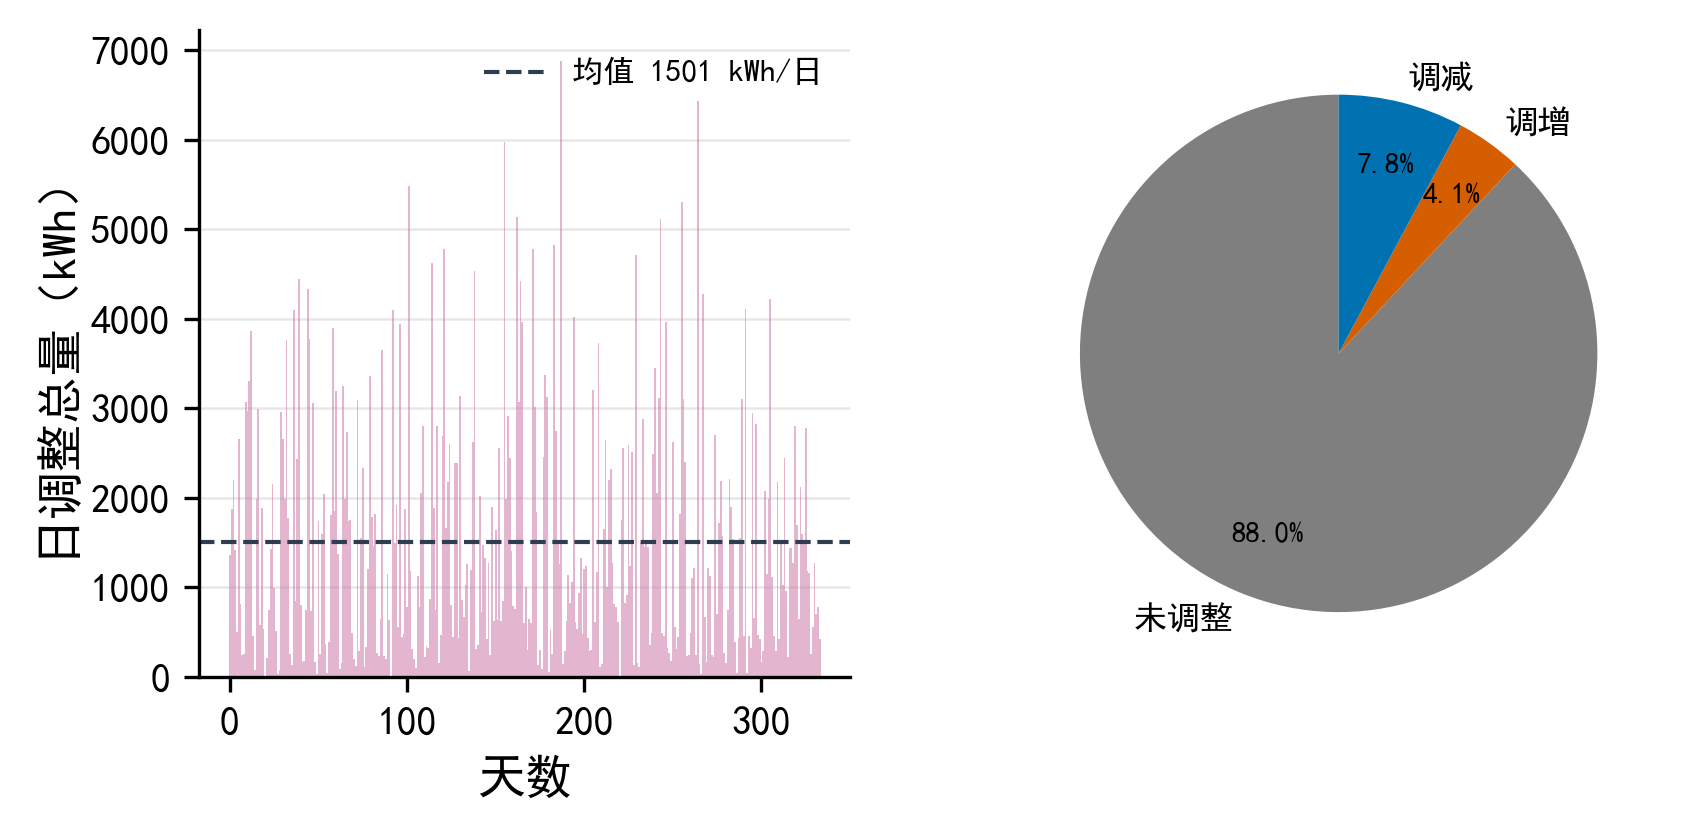
\includegraphics[width=0.92\textwidth]{figures/fig_val_adj_dist.png}
  \caption{问题三全年调整量统计：(a) 逐日调整总量；(b) 调整方向占比}
  \label{fig:val_adj}
\end{figure}

\begin{table}[H]
  \centering
  \caption{问题三指定日期的（最终）购电量（按表1格式，单位 kWh）}
  \label{tab:q3dates1}
  \begin{tabularx}{0.94\textwidth}{C{0.16\textwidth} R R R R}
    \toprule
    时间段 & 2025.3.20 & 2025.6.21 & 2025.9.23 & 2025.12.21 \\
    \midrule
    10:00--10:10 & 0.00 & 0.00 & 0.00 & 0.00 \\
    12:00--12:10 & 535.88 & 0.00 & 316.99 & 862.45 \\
    14:00--14:10 & 0.00 & 0.00 & 0.00 & 0.00 \\
    16:00--16:10 & 480.62 & 65.00 & 400.23 & 859.33 \\
    18:00--18:10 & 713.13 & 428.85 & 750.65 & 704.39 \\
    20:00--20:10 & 0.00 & 0.00 & 18.41 & 0.00 \\
    \midrule
    全天购电量 & 65,626.93 & 36,256.89 & 64,283.38 & 95,412.03 \\
    全天偏差结算费/元 & 41,003.83 & 20,708.21 & 40,452.00 & 61,930.32 \\
    紧急购电费/元 & 4,460.58 & 0.00 & 8,650.02 & 0.00 \\
    \bottomrule
  \end{tabularx}
\end{table}

\begin{table}[H]
  \centering\footnotesize\setlength{\tabcolsep}{3pt}
  \caption{问题三指定日期的储能充放电量与储电量（按表2格式，单位 kWh）}
  \label{tab:q3dates2}
  \begin{tabularx}{0.98\textwidth}{C{0.115\textwidth} R R R R R R R R}
    \toprule
    & \multicolumn{2}{c}{2025.3.20} & \multicolumn{2}{c}{2025.6.21} & \multicolumn{2}{c}{2025.9.23} & \multicolumn{2}{c}{2025.12.21} \\
    \cmidrule(lr){2-3}\cmidrule(lr){4-5}\cmidrule(lr){6-7}\cmidrule(lr){8-9}
    时间段 & 充电 & 放电 & 充电 & 放电 & 充电 & 放电 & 充电 & 放电 \\
    \midrule
    0:00--4:00 & 232.37 & 0.00 & 152.96 & 3150.39 & 891.59 & 349.61 & 1103.92 & 363.12 \\
    4:00--8:00 & 179.47 & 5574.77 & 203.21 & 5378.29 & 845.86 & 5609.07 & 1295.52 & 825.33 \\
    8:00--12:00 & 3180.77 & 3210.61 & 10134.27 & 0.00 & 4295.05 & 2387.94 & 4422.29 & 8101.09 \\
    12:00--16:00 & 6847.14 & 254.72 & 91.76 & 0.00 & 6316.01 & 403.62 & 8337.69 & 2234.49 \\
    16:00--20:00 & 652.22 & 4827.08 & 85.45 & 4761.23 & 0.00 & 4755.61 & 13.62 & 4942.37 \\
    20:00--24:00 & 9911.14 & 3617.70 & 9873.05 & 3305.15 & 8734.20 & 3884.39 & 9905.09 & 3659.08 \\
    \midrule
    0:00 / 24:00 储电量 & \multicolumn{2}{c}{10590.86 / 10066.03} & \multicolumn{2}{c}{10752.34 / 10800.00} & \multicolumn{2}{c}{9408.84 / 9060.78} & \multicolumn{2}{c}{9961.01 / 10169.67} \\
    \bottomrule
  \end{tabularx}
\end{table}

\begin{table}[H]
  \centering
  \caption{问题三指定日期的紧急购电量（按表3格式，单位 kWh）}
  \label{tab:q3emg}
  \begin{tabularx}{0.8\textwidth}{C{0.2\textwidth} C{0.28\textwidth} R}
    \toprule
    日期 & 紧急购电时间段 & 紧急购电量 \\
    \midrule
    2025.3.20 & 0:20--0:50 & 107.84 \\
     & 1:10--2:20 & 214.88 \\
     & 2:40--4:00 & 338.87 \\
     & 5:50--6:00 & 18.50 \\
     & 7:10--7:40 & 97.30 \\
     & 9:50--10:10 & 54.95 \\
     & 16:00--16:20 & 483.50 \\
     & 18:20--18:30 & 4.26 \\
     & 20:20--20:30 & 50.30 \\
    \midrule
    2025.6.21 & \multicolumn{2}{c}{无紧急购电} \\
    \midrule
    2025.9.23 & 0:30--1:10 & 174.64 \\
     & 15:00--15:20 & 610.47 \\
     & 16:00--17:10 & 350.59 \\
     & 17:40--19:00 & 361.75 \\
     & 20:20--20:40 & 69.88 \\
     & 21:00--22:00 & 445.54 \\
    \midrule
    2025.12.21 & \multicolumn{2}{c}{无紧急购电} \\
    \bottomrule
  \end{tabularx}
\end{table}

\begin{figure}[H]
  \centering
  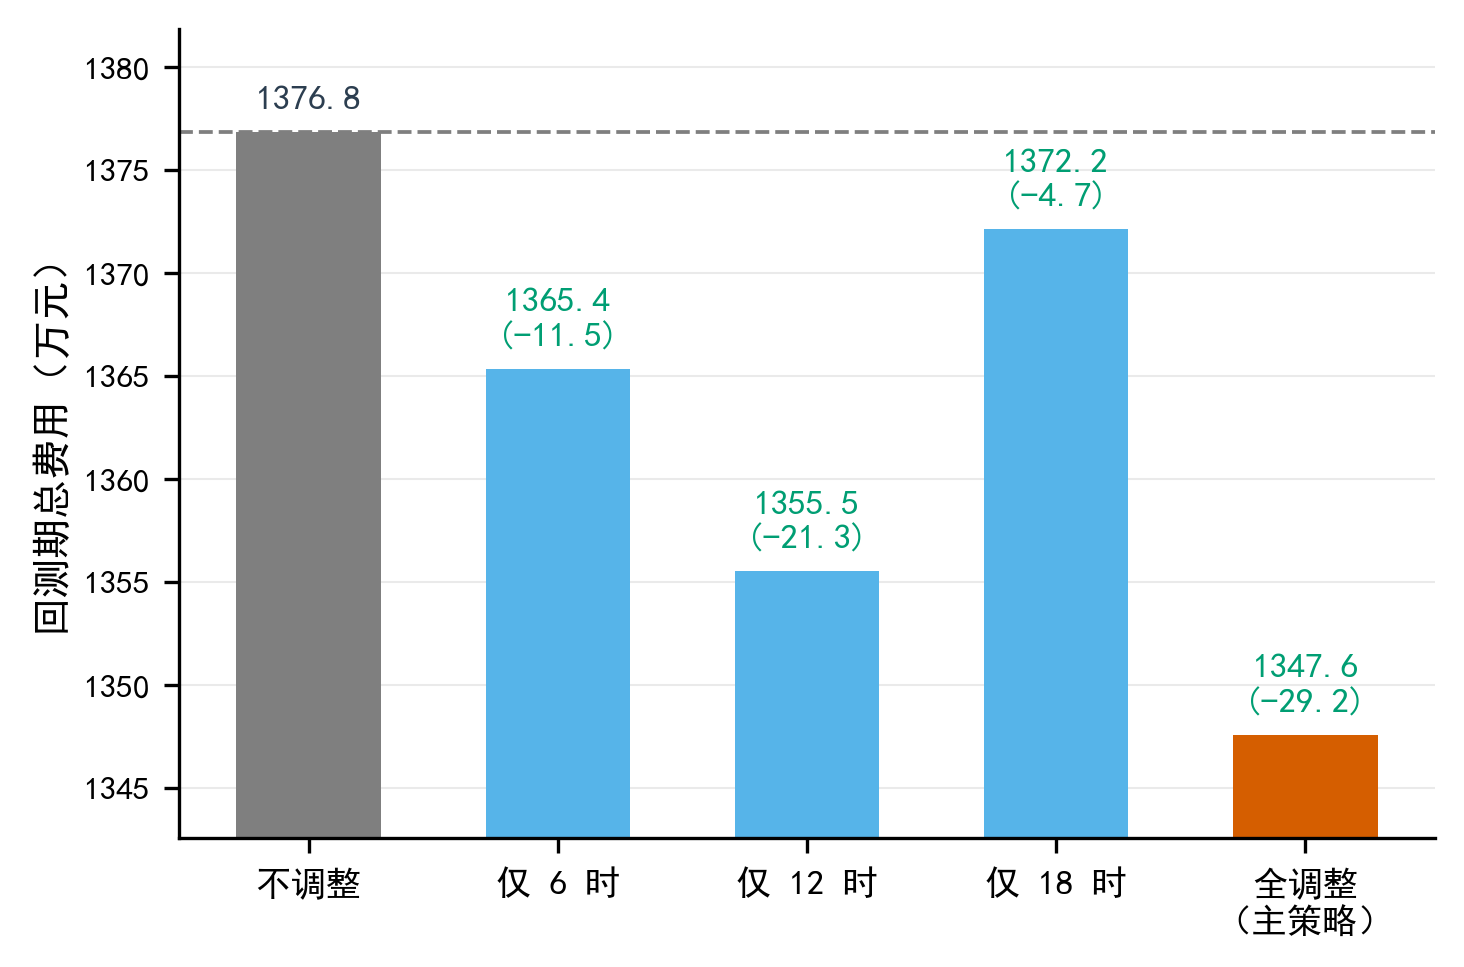
\includegraphics[width=0.78\textwidth]{figures/fig_q3_adj_cmp.png}
  \caption{问题三：各调整策略总费用对比}
  \label{fig:q3cmp}
\end{figure}

\begin{figure}[H]
  \centering
  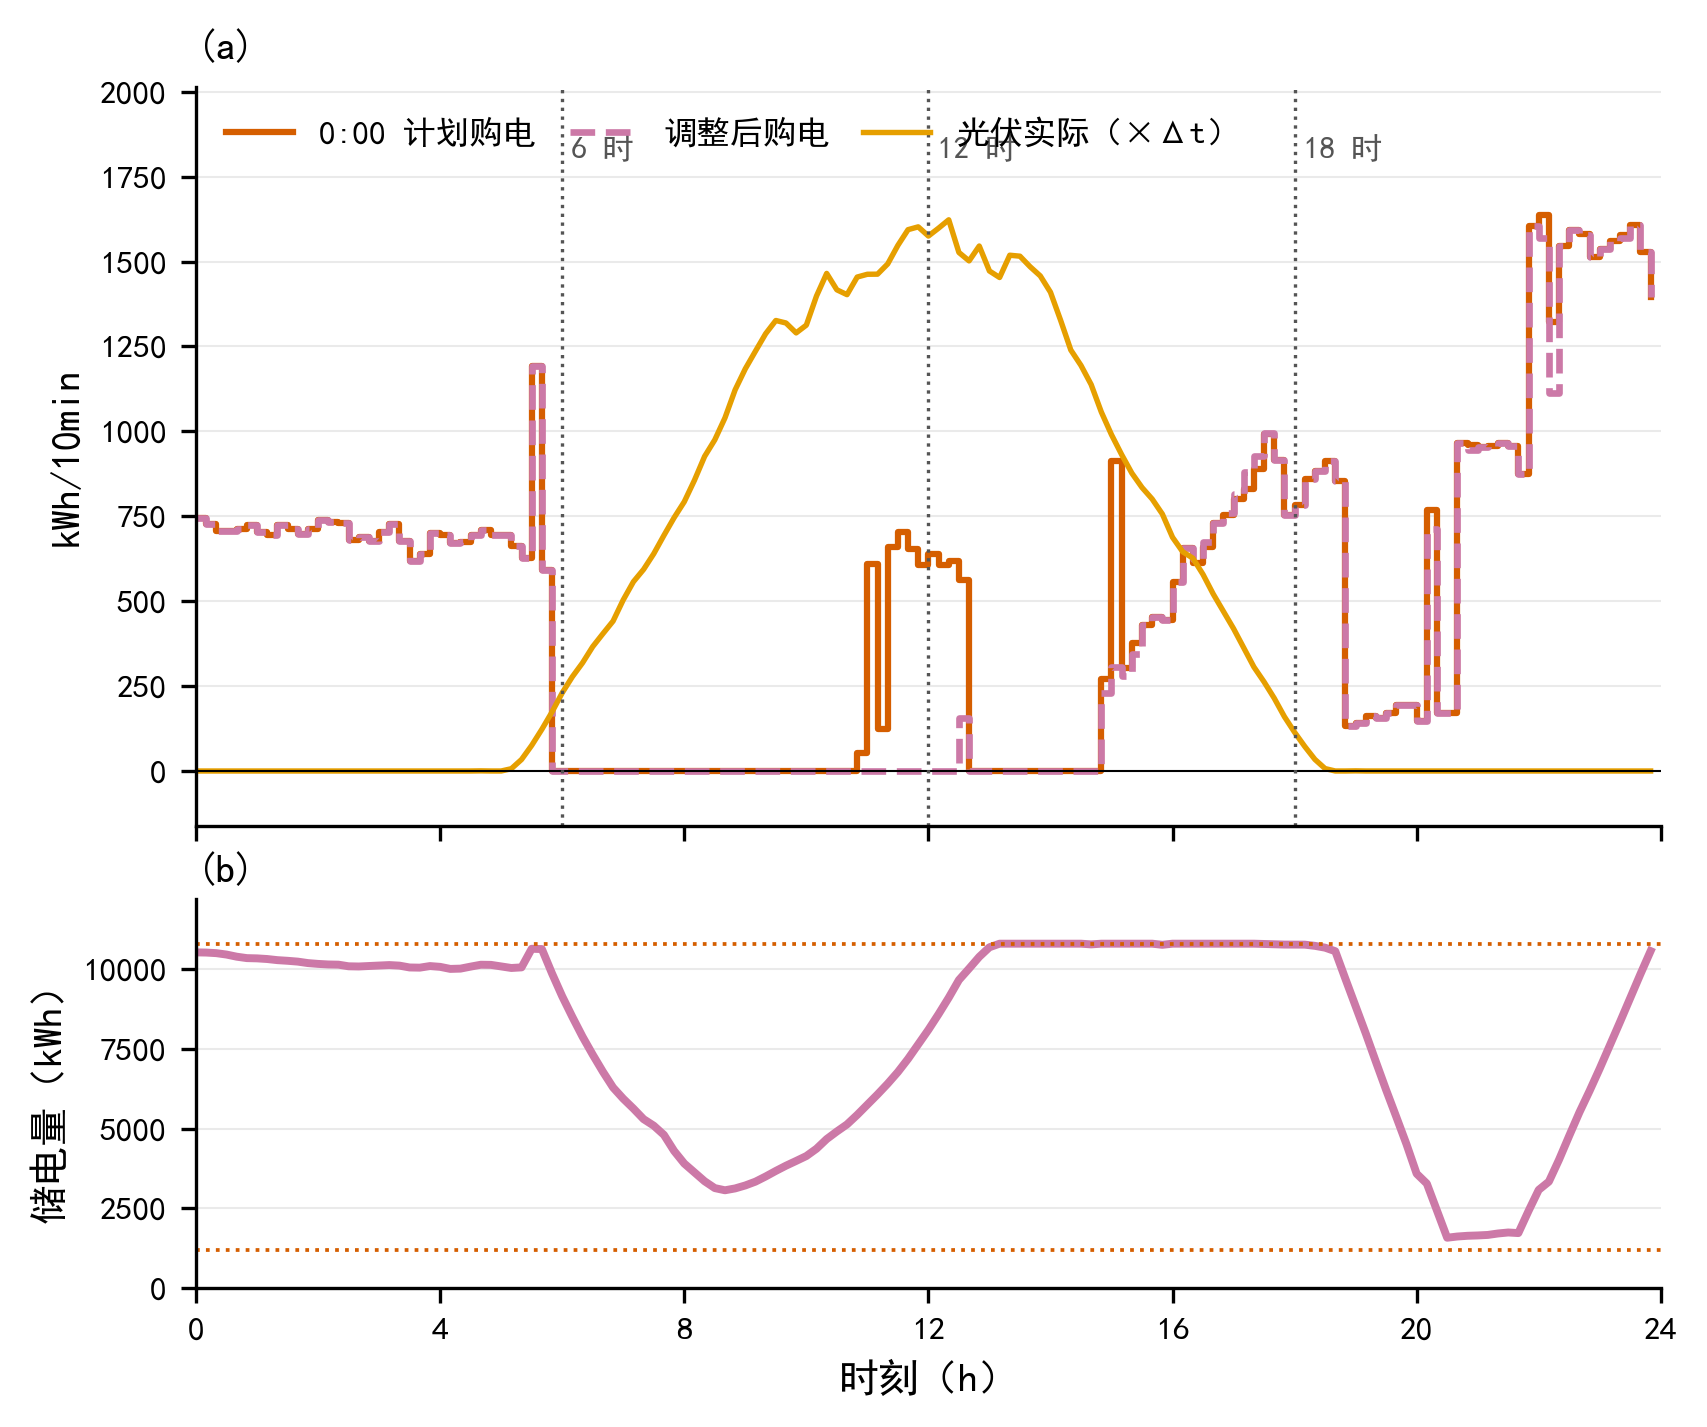
\includegraphics[width=0.95\textwidth]{figures/fig_q3_adj_day.png}
  \caption{滚动调整示例（2025.10.23，调整总量最大日）：(a) 0:00 计划购电、调整后购电与光伏实际出力，竖虚线为三次预报时刻；(b) 储电量轨迹}
  \label{fig:q3day}
\end{figure}

完整结果见支撑材料 \texttt{result3.xlsx}（334 天逐时段计划购电量、调整购电量、充放电量与紧急购电记录）。

\section{问题四：波动电价下的购电模型}

\subsection{建模准备}

附件4 电价全年实时波动，范围 0.0076--1.7936 元/kWh（附件1 固定电价范围为 0.3713--1.3952 元/kWh），峰谷价差显著拉大且出现近零电价时段。本文按\textbf{日前已知}处理当日电价路径，这是\textbf{额外的信息假设}：题目原文仅称``电价实时波动''并要求根据附件4重算，未明确 0:00 是否能获取全天电价路径。本文采用该假设的理由是：日前市场出清价于运营日前发布是电力市场常见惯例，且题目的结算规则均按``交易时刻电价''计价。在此信息结构下，问题二、三的全部机制保持不变，仅将电价序列替换为附件4。\textbf{若电价亦不可预知}，需引入电价预测模型（如基于历史同期价格的加权估计），计划与调整的 LP 将使用预测电价、结算使用实际电价，预计总费用将高于当前报告值。将附件4 换回附件1，模型即退化为问题二/三（同一代码路径），退化一致性检验通过。

\subsection{结果与分析}

固定电价与波动电价下各策略的回测期总费用对比见表~\ref{tab:q4cmp}与图~\ref{fig:q4cmp}。

\begin{table}[H]
  \centering
  \caption{固定电价（附件1）与波动电价（附件4）下各策略总费用对比（万元）}
  \label{tab:q4cmp}
  \begin{tabularx}{0.86\textwidth}{L R R R}
    \toprule
    策略 & 固定电价 & 波动电价 & 变化幅度 \\
    \midrule
    无储能基准 & 1640.7 & 1702.7 & $+3.8\%$ \\
    问题二模型（P4-2） & 1387.9 & 1460.8 & $+5.3\%$ \\
    问题三模型（不调整） & 1376.8 & 1446.9 & $+5.1\%$ \\
    \textbf{问题三模型（全调整，P4-3 主策略）} & \textbf{1347.6} & \textbf{1414.5} & $+5.0\%$ \\
    理想先知 & 1224.5 & 1283.0 & $+4.8\%$ \\
    \bottomrule
  \end{tabularx}
\end{table}

波动电价使各策略总费用普遍上升 4\%--5\%，但两点结构性观察表明模型对电价体制稳健：

\textbf{（1）储能套利空间扩大。}附件4 出现 0.0076 元/kWh 的近零电价时段（不足固定电价低谷 0.43 元/kWh 的 2\%），主策略在这些时段近乎免费充电、并在 1.79 元/kWh 的高价时段深度放电。波动电价下主策略较无储能基准节省 \textbf{288.13 万元（16.9\%）}，与固定电价下的降幅（16.9\%）持平。

\textbf{（2）调整价值放大。}波动电价下场景化滚动调整较不调整节省 \textbf{32.41 万元}（固定电价下为 29.25 万元）。偏差结算按交易时刻电价计价，低价时段调减（按 50\% 退款）与高价时段规避紧急购电（5 倍价）的价值均随价格波动增大；同时信息融合的贡献亦由 14.0 万元升至 17.2 万元。

计划层场景数沿用 $S=10$：波动电价下 $S \in \{10,14\}$ 的总费用为 1463.6 / 1471.4 万元，与固定电价下的选择一致，超参数稳健。指定日期的汇总结果见表~\ref{tab:q4dates}（逐时段明细见支撑材料 \texttt{result4-2.xlsx} 与 \texttt{result4-3.xlsx}）。

\begin{table}[H]
  \centering
  \caption{问题四（P4-3 主策略）指定日期结果汇总}
  \label{tab:q4dates}
  \begin{tabularx}{0.9\textwidth}{C{0.16\textwidth} R R R R}
    \toprule
    日期 & 全天购电量/kWh & 偏差结算费/元 & 紧急购电费/元 & 调整总量/kWh \\
    \midrule
    2025.3.20 & 66,126.86 & 41,734.46 & 4,047.20 & 3,135.41 \\
    2025.6.21 & 37,175.15 & 18,491.53 & 0.00 & 315.74 \\
    2025.9.23 & 65,856.06 & 42,828.76 & 5,584.16 & 1,397.45 \\
    2025.12.21 & 95,582.93 & 72,584.42 & 0.00 & 1,699.05 \\
    \bottomrule
  \end{tabularx}
\end{table}

\begin{figure}[H]
  \centering
  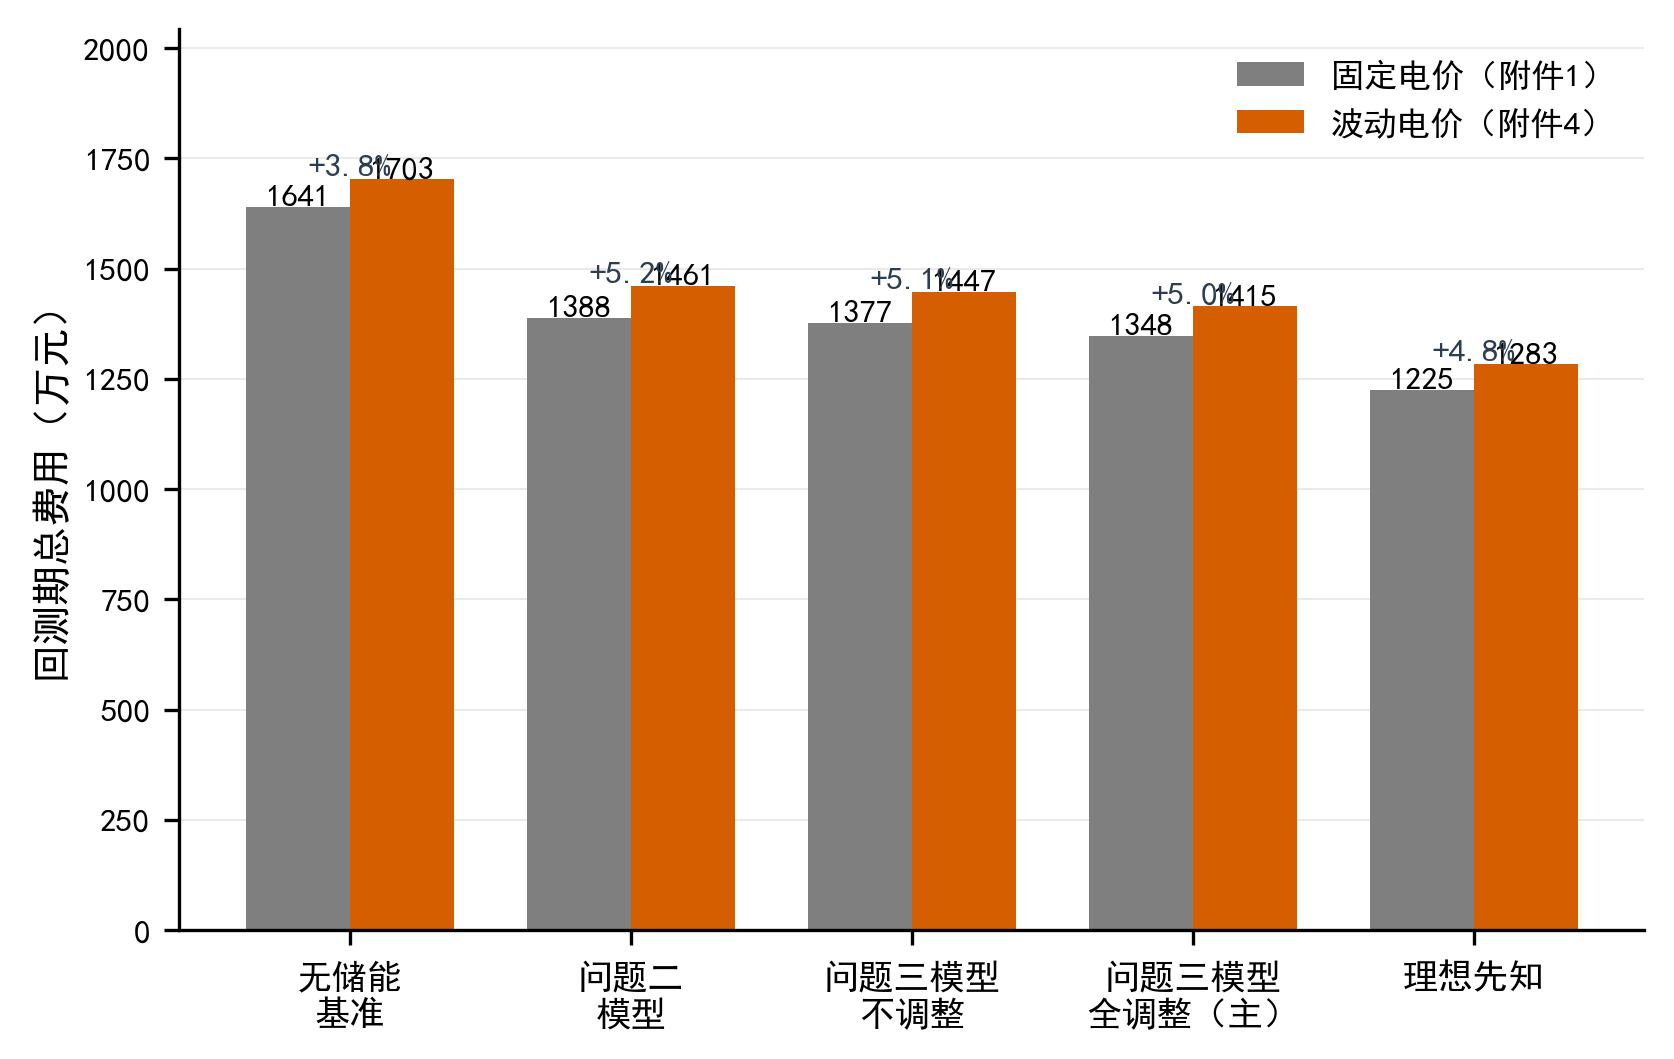
\includegraphics[width=0.95\textwidth]{figures/fig_q4_cmp.png}
  \caption{固定电价与波动电价下各策略总费用对比}
  \label{fig:q4cmp}
\end{figure}

\section{灵敏度分析}

为检验模型与结论对关键参数的稳健性，围绕储能效率、荷电状态安全区间与紧急购电惩罚倍数开展敏感性分析；缓冲分位数与偏差结算口径的敏感性已分别在问题二、三中给出。

\textbf{（1）充放电效率。}效率 $\eta$ 在 $0.85 \sim 0.95$ 内变动时，问题一日购电费由 36603.21 元单调降至 33767.02 元（$\eta{=}0.9$ 时 35126.85 元），平均每提升 0.01 效率节省约 284 元；问题二回测期总费用由 1470.5 万元降至 1369.0 万元，变化幅度约 $\pm 3.4\%$。效率只影响套利空间的大小，不改变``低谷充电、高峰放电''的最优策略结构。

\textbf{（2）荷电状态安全区间。}下限由 1200 降至 960 kWh（或升至 1440），问题一购电费仅变化 $-0.45\%$/$+0.46\%$；上限由 10800 降至 8640 kWh 时购电费上升 5.12\%（问题二上升 5.05\%），升至物理容量 12000 kWh 时下降 2.24\%。说明模型对下限不敏感，而上限（即可用储能容量）是经济性的主导参数——这为储能容量配置提供了直接依据：在当前峰谷价差下，扩充储能上限的边际价值显著。

\textbf{（3）紧急购电惩罚倍数。}惩罚倍数 $m$ 由 3 增至 8 时（图~\ref{fig:sens}(c)），问题二总费用（固定 $q{=}0.7$）由 1374.0 万元升至 1480.5 万元；若按报童理论随 $m$ 重选分位数 $q^* = (m-1)/m$，费用可降至 1442.7 万元（$m{=}8$ 时节省 37.8 万元）。$m$ 越大，缓冲的价值越高，且理论最优分位数与实测最优值始终保持一致（$m{=}5$ 时 $q^*{=}0.8$，实测最优区间 $[0.7,0.8]$），验证了式~\eqref{eq:newsvendor} 的正确性。

\begin{figure}[H]
  \centering
  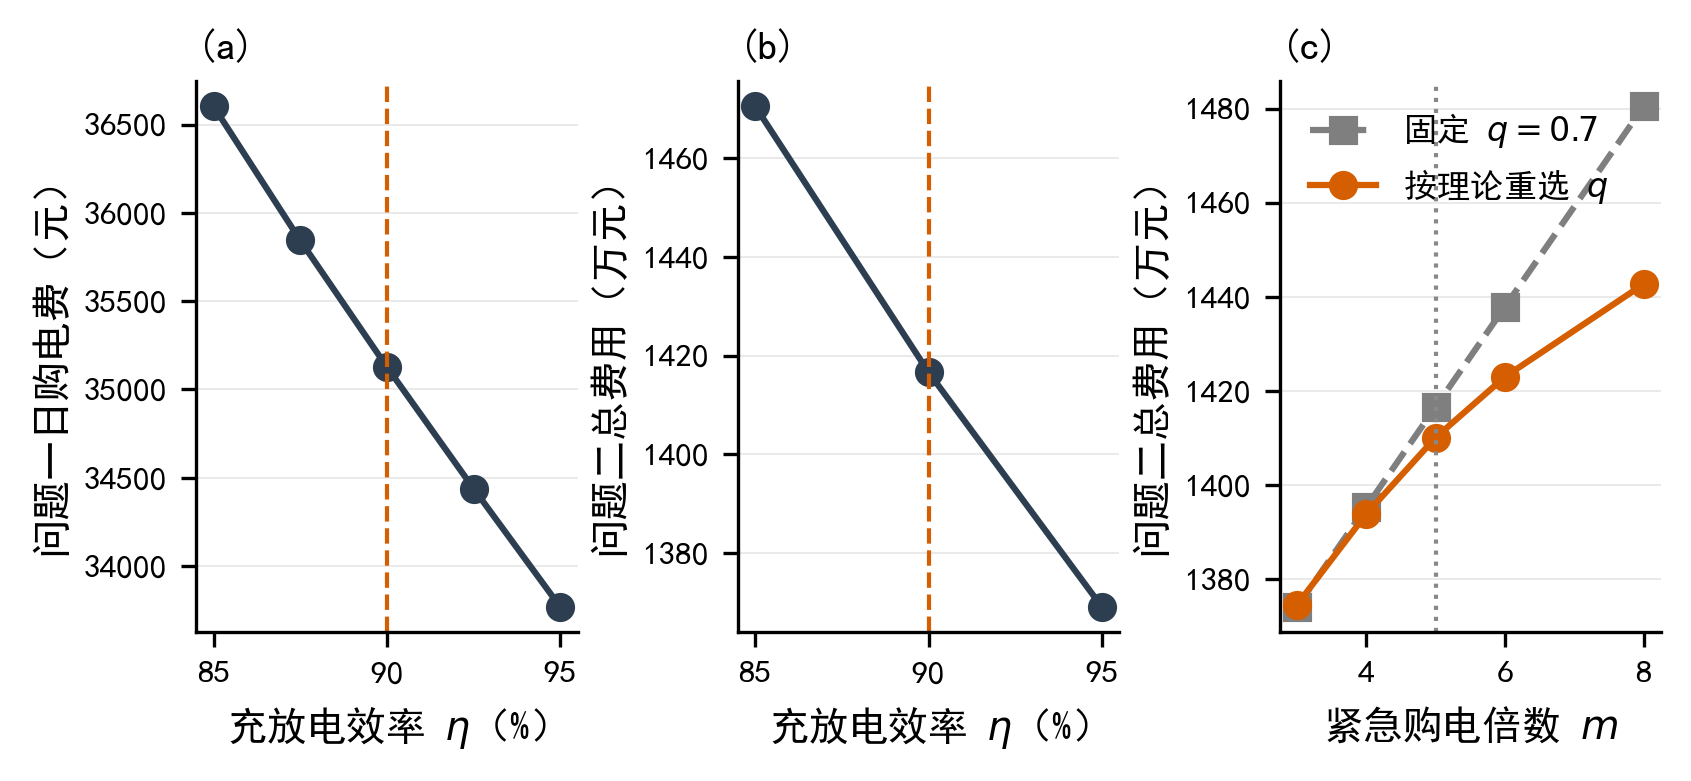
\includegraphics[width=0.98\textwidth]{figures/fig_sens.png}
  \caption{灵敏度分析：(a)(b) 充放电效率对问题一/二费用的影响；(c) 紧急购电倍数与缓冲分位数重选}
  \label{fig:sens}
\end{figure}

\section{模型评价与推广}

\textbf{优点：}
\begin{enumerate}
  \item \textbf{统一的多层随机优化框架}：计划层与调整层均为两阶段随机规划（场景法），执行层为滚动实时线性规划——风险刻画全链条一致，且实验证明了视角一致性对调整价值的决定性作用；
  \item \textbf{全局最优保证}：各层均为线性规划，HiGHS 求解器求得全局最优——九组替代策略对照实验（含 CVaR-SAA 与全时域 MPC）进一步验证了期望最优框架的正确性；
  \item \textbf{严格因果}：预测只用历史数据、场景只用滞后误差、仿真内置信息集约束——杜绝数据泄漏；
  \item \textbf{理论支撑完备}：报童分位数缓冲是 SAA 在无储能单时段下的特例（理论 $q^*=0.8$ 与实测最优区间 $[0.7,0.8]$ 一致）；对偶分析给出边际供电成本与储能容量影子价格；
  \item \textbf{信息融合增益}：官方预报与历史均值的按均方误差倒数加权组合将光伏预测 MAE 降低 35\%（197.5 $\to$ 127.8 kW）；
  \item \textbf{完全可复现}：全部结果由代码自动校验（平衡残差、SOC 区间、循环条件）并落盘为单一数据源，九组对照实验的代码全部入库。
\end{enumerate}

\textbf{缺点：}
\begin{enumerate}
  \item SAA 场景集取近 10 天误差曲线的等概率经验分布，未刻画误差的时间自相关与条件结构；
  \item 执行层滚动优化沿用 0:00 的负载预测，未利用日内已发生的实际值修正（实验证明自适应修正反而恶化）；
  \item 问题四假设电价日前已知；若电价亦需实时预测，需引入价格预测模型；
  \item 预测器未利用气象协变量（题目未提供），多云天气下的光伏突变预测能力有限。
\end{enumerate}

\textbf{推广：}本框架可直接推广至含风电机组的微网、多微网共享储能的分布式调度（增加耦合约束即可保持线性）；将经验场景集升级为条件场景生成或分布鲁棒优化，可进一步刻画误差的结构性依赖；对偶分析给出的储能容量影子价格可直接用于容量投资决策。

% 2026 强制要求：AI 工具使用声明必须置于参考文献之前，以下二选一。
% \CumcmAINotUsed
\CumcmAIUsed{建模思路讨论、代码编写与调试、数据分析与论文初稿撰写}

\bibliographystyle{gbt7714-numerical}
\bibliography{references}

\newpage
\appendix
\titleformat{\section}
  {\centering\heiti\zihao{3}\bfseries}
  {附录~\thesection}
  {0.8em}
  {}

\section{支撑材料文件列表}

%% TODO-FINAL：提交前与实际压缩包逐项核对
\begin{longtable}{@{}p{0.08\textwidth}p{0.36\textwidth}p{0.44\textwidth}@{}}
  \toprule
  序号 & 文件路径 & 内容说明 \\
  \midrule
  1 & \texttt{code/common.py} & 公共模块：数据加载、时间约定、LP 求解器 \\
  2 & \texttt{code/q1\_plan\_lp.py} & 问题一：日循环线性规划求解与 result1 输出 \\
  3 & \texttt{code/q2\_forecast.py} & 问题二：负载/光伏预测器对比 \\
  4 & \texttt{code/q2\_simulate.py} & 问题二：全年计划-执行仿真与策略对比 \\
  5 & \texttt{code/q2\_results.py} & 问题二：result2.xlsx 输出与图表 \\
  6 & \texttt{code/q3\_simulate.py} & 问题三：滚动调整仿真与策略对比 \\
  7 & \texttt{code/q3\_results.py} & 问题三：result3.xlsx 输出与图表 \\
  8 & \texttt{code/q4\_simulate.py} & 问题四：波动电价下的重算 \\
  9 & \texttt{code/q4\_results.py} & 问题四：result4-2/4-3.xlsx 输出与图表 \\
  10 & \texttt{code/xlsx\_writer.py} & 结果工作簿写出公共模块 \\
  11 & \texttt{code/sens\_analysis.py} & 全局灵敏度分析 \\
  12 & \texttt{code/q2\_saa.py} & 问题二两阶段随机规划（SAA） \\
  13 & \texttt{code/figstyle.py}、\texttt{code/restyle\_figures.py} & 图表统一风格与生成 \\
  14 & \texttt{code/q2\_variants.py}、\texttt{} & 对照实验：场景选择、分位数变体池、信息价值分解 \\
  15 & \texttt{code/q2\_cvar.py}、\texttt{code/q2\_mpc.py} & 证伪实验：CVaR-SAA 网格、全时域 MPC 执行 \\
  16 & \texttt{code/q2\_fc2\_test.py}、\texttt{code/q2\_final.py} & 证伪实验：预测器变体、加权场景池 \\
  17 & \texttt{code/fig\_new.py} & 新增图表：EDA 热力图/箱线/分布、模型验证/全年轨迹/月度分解 \\
  18 & \texttt{results/result1.xlsx} $\sim$ \texttt{result4-3.xlsx} & 四问完整结果文件 \\
  \bottomrule
\end{longtable}

\section{完整源程序}

\lstinputlisting[language=Python,basicstyle=\ttfamily\scriptsize,breaklines=true,breakatwhitespace=false,caption={公共模块 common.py}]{code/common.py}
\lstinputlisting[language=Python,basicstyle=\ttfamily\scriptsize,breaklines=true,breakatwhitespace=false,caption={问题一求解程序 q1\_plan\_lp.py}]{code/q1_plan_lp.py}
\lstinputlisting[language=Python,basicstyle=\ttfamily\scriptsize,breaklines=true,breakatwhitespace=false,caption={问题二预测程序 q2\_forecast.py}]{code/q2_forecast.py}
\lstinputlisting[language=Python,basicstyle=\ttfamily\scriptsize,breaklines=true,breakatwhitespace=false,caption={问题二仿真程序 q2\_simulate.py}]{code/q2_simulate.py}
\lstinputlisting[language=Python,basicstyle=\ttfamily\scriptsize,breaklines=true,breakatwhitespace=false,caption={问题二两阶段随机规划 q2\_saa.py}]{code/q2_saa.py}
\lstinputlisting[language=Python,basicstyle=\ttfamily\scriptsize,breaklines=true,breakatwhitespace=false,caption={问题二结果输出 q2\_results.py}]{code/q2_results.py}
\lstinputlisting[language=Python,basicstyle=\ttfamily\scriptsize,breaklines=true,breakatwhitespace=false,caption={问题三仿真程序 q3\_simulate.py}]{code/q3_simulate.py}
\lstinputlisting[language=Python,basicstyle=\ttfamily\scriptsize,breaklines=true,breakatwhitespace=false,caption={问题三结果输出 q3\_results.py}]{code/q3_results.py}
\lstinputlisting[language=Python,basicstyle=\ttfamily\scriptsize,breaklines=true,breakatwhitespace=false,caption={问题四仿真程序 q4\_simulate.py}]{code/q4_simulate.py}
\lstinputlisting[language=Python,basicstyle=\ttfamily\scriptsize,breaklines=true,breakatwhitespace=false,caption={问题四结果输出 q4\_results.py}]{code/q4_results.py}
\lstinputlisting[language=Python,basicstyle=\ttfamily\scriptsize,breaklines=true,breakatwhitespace=false,caption={结果写出公共模块 xlsx\_writer.py}]{code/xlsx_writer.py}
\lstinputlisting[language=Python,basicstyle=\ttfamily\scriptsize,breaklines=true,breakatwhitespace=false,caption={灵敏度分析 sens\_analysis.py}]{code/sens_analysis.py}
\lstinputlisting[language=Python,basicstyle=\ttfamily\scriptsize,breaklines=true,breakatwhitespace=false,caption={图表风格模块 figstyle.py}]{code/figstyle.py}
\lstinputlisting[language=Python,basicstyle=\ttfamily\scriptsize,breaklines=true,breakatwhitespace=false,caption={图表生成程序 restyle\_figures.py}]{code/restyle_figures.py}

\end{document}
